% !TeX option = --shell-escape
\documentclass{article}
\usepackage{graphicx}
\usepackage{amsmath}
\usepackage{mathtools}
\usepackage{hyperref}
\usepackage{here}
\usepackage{verbatim}
\usepackage{mhchem}
\usepackage{minted}
%\usepackage{nccmath}
\setcounter{MaxMatrixCols}{20}
\usepackage[utf8]{inputenc}
\usepackage[english]{babel}
\usepackage{csquotes} % Consigliato per la gestione delle citazioni
\usepackage[utf8]{inputenc}
\usepackage[english]{babel}
\usepackage{csquotes} % Consigliato per la gestione delle citazioni

\usepackage[english]{babel}
\usepackage{csquotes} % Consigliato per la gestione delle citazioni


\usepackage[utf8]{inputenc}
\usepackage{biblatex} %Imports biblatex package
\addbibresource{ref.bib} %Import the bibliography file
\title{Species invasion and autocatalysis}
%\author{Simone Cavallero }
\date{May 2024}
\begin{document}

\maketitle

\section{Introduction}
Let us consider a population of original species $X$, which is subject to invasion from invader species $Y$. The concentration of species $X$ is assumed to remain constant during the invasion of species $Y$. The $X$ species are in number $N_X$ and the $Y$ species in number $N_Y$. We assume that species $X$ and $Y$ are part of a network with randomly chosen topology defined by a stoichiometric matrix. In addition, random parameters are used to specify the kinetics.  We want to know whether the capacity of the invaders $Y$ to grow dynamically into an existing population of $X$ is related to its ability to build autocatalytic networks with the species already present. 

\section{Construction of a chemical network with random topology}
\subsection{Stochiometric matrices}
Let $S$ be the stoichiometric matrix of the system of both species $X$ and $Y$, which  includes a total number of reactions $N_R$. Let $S_P$ a be a submatrix of $S$, which describes only the evolution of $Y$ species within the $N_R$ reactions. Hence, $S_P$ is and $S \in Z^{(N_X+N_Y) \times N_R}$ and 
$S_P \in  Z^{N_Y \times N_R}$.

All reactions are assumed as reversible unless specified otherwise. To construct the random $S$ matrix, we split it into its forward and backward components:
\begin{equation}
    S= S_- - S_+
\end{equation}
First, we require that the total order of the forward and backward reactions is separately smaller than 2. For both forward and backward reactions, a random integer between 0 and 2 sets this total order. We then assign randomly for each forward reaction, the species that will participate in it, until the total forward order is attained. Once the random matrix $S_+$ is built in that way, we do the same for the backward reactions, thus constructing $S_-$. Depending on the choice of \textbf{dilution}, \textbf{ambiguity} and \textbf{autonomy} conditions, we put constraints on species participating in the reactions.

\subsection{Autonomy}\label{aut}
The first condition we usually require for our reactions, is that we always need at least one $Y$ species as a reactant and one as a product. It does not matter whether $X$ species participate in the reactions as far as we have one $Y_i$ and one $Y_j$ as reactant and product, the autonomy condition is satisfied. With autonomy, the allowed reactions are of the following types :
\begin{equation}
\label{set_reactions}
		\begin{split}
		\ce{\textsf{Y}_i & <--> \textsf{Y}_j } \\ 
\ce{\textsf{Y}_i & <--> \textsf{Y}_j + \textsf{Y}_k} \\ \ce{\textsf{Y}_i + \textsf{X}_l & <--> \textsf{Y}_j + \textsf{X}_m}.	
		\end{split} 
\end{equation}

When the autonomy condition is instead \textbf{non-satisfied}, we also allow  degradation reactions in which \textbf{no Y species exist as product}. Note that $Y$ is in any case always required as a reactant. Thus, reactions of the following type are allowed :
\begin{equation}
\begin{split}
\ce{\textsf{Y}_i & -> $\emptyset$ } \\ 
\ce{\textsf{Y}_i +\textsf{Y}_j  & -> $\emptyset$}\\ 
\ce{\textsf{X}_l +\textsf{Y}_i  & -> $\emptyset$}.
\end{split} 
\end{equation}
Note that in that case, these reactions are not reversible.

%\small{NOTE: NON-AUTONOMY CAN BE ALLOWED ONLY WHEN WE ARE NOT IN A DILUTED SYSTEM. IF DILUTED IS SET TO "TRUE", THERE'S NO POSSIBILITY TO HAVE AUTONOMY SET TO "FALSE" AS WELL.}

\subsection{Dilution (TOP)}\label{deg}
When the system is diluted, reactions involving 2 or more reactants among $Y$ species are negligible \cite{2}. 
Importantly, we also enforce the autonomy condition in our definition of "diluted" systems. This corresponds to the TOP condition introduced in \cite{2}, which is applicable to \textbf{diluted and autonomous} systems, in which the allowed reactions are of the types :
\begin{equation}
		\begin{split}
\ce{\textsf{Y}_i & <--> \textsf{Y}_j } \\ 
\ce{\textsf{Y}_i & -> s_1 \textsf{Y}_{j1} + s_2 \textsf{Y}_{j2} + .. } \quad \quad \sum_l s_l \ge 2 \\ 
\end{split} 
\end{equation}


\subsection{Ambiguity}\label{amb}
Ambiguous reactions are reactions in which the same species are present as a product and as a reactant, which is frequently the case in catalytic reactions. If ambiguity is instead forbidden, then if a species appears as reactant, it cannot be selected as a product and vice-versa, which means that  only the following types of reactions are allowed :
\begin{equation}
		\begin{split}
\ce{\textsf{Y}_i & <--> \textsf{Y}_j } \quad \quad i \neq j \\ 
\ce{\textsf{Y}_i & <--> \textsf{Y}_j + \textsf{Y}_k } \quad \quad i \neq j,k \\ 
\ce{\textsf{Y}_i + \textsf{Y}_j & <--> \textsf{Y}_k + \textsf{Y}_l } \quad \quad i,j \neq k,l \\ 
\ce{\textsf{X}_l + \textsf{Y}_i & <--> \textsf{Y}_j + \textsf{X}_m } \quad \quad i \neq j \\ 
\end{split} 
\end{equation}


\section{Simulation Setup}
We develop a code that builds and analyze many random chemical networks. Their stoichiometric matrices are randomly constructed based on the choice of
Autonomy, Dilution (TOP) and Ambiguity.

We build it upon an existing code developed by \cite{3}, from which we extract a function that is able to find autocatalytic cores inside the network of the invaders and another function that identifies those cores and computes their eigenvalues.
Then, we define the main function with all the parameters it needs, where "law" corresponds to the chosen rate law, "MAL" for mass-action law and "MM" for Michaelis-Menten (actually Hill) type. Backward reactions are always set to be of the MAL type.
Note that $S_+$ and $S_-$ are called in the code $S$ and $S1$. We also set the initial condition for the $X$ and $Y$ vectors and randomize the forward rate constants.\\

For thermodynamic consistency, we randomize the vector of the standard chemical potentials $\pmb{\mu}_0$. Indeed, for each reaction we need to fulfill \textbf{detailed local balance}:

\begin{center}
    \begin{equation}
        \log \frac{k_{+i}}{k_{-i}} = -\Delta G_0 = - S^T \pmb{\mu}_0 \quad \forall i \in 1, . . ., N_R
    \end{equation}
\end{center}

Since the set of forward constants and the vector of standard chemical potentials are randomly chosen, the backward rates will be computed as 

\begin{center}
    \begin{equation}
       k_{-i} = k_{+i} e^{\Delta G_0} = e^{S^T\pmb{\mu}_0} \quad \forall i \in 1, . . ., N_R
    \end{equation}
\end{center}




The next part of the code is devoted to the random construction of the matrices $S$ and $S_P$ according to the choice of autonomy, dilution and ambiguity. Then, $S_P$ is extracted from $S$, since it is a submatrix of it. The autocatalytic detection code is called on the matrix of the invaders, to check whether autocatalysis is present or not.

The autocatalytic detection code, is constructed in such a way that it will analyze all the cores found inside the invaders' network, as well as determining if autocatalysis is present or not. If the "REALIZATION" is indeed autocatalytic, it will be saved as "True" in the autocatalytics vector, otherwise as false. The "stoichio" function will then construct the cores from the matrix and perform permutations to transform them into Metzler matrices. Then, as explained in \cite{1}, we can check if they are instable.


Afterwards, the simulation of the systems starts, and records the time series of the $Y$'s, $S$ and $S_P$ and indicate above these, in the same file, whether their system was autocatalytic or not. We then proceed to establish the survival of the population, which is defined as the ability to pass a given threshold. This ends the main function, which returns the ordered vector of autocatalytic systems and the ordered vector of survival ones.

\section{Numerical detection of stoichiometric autocatalysis}

One may argue whether the cores themselves are the cause of the exponential growth in the network, which we call the dynamical autocatalysis. If they are, one might expect the Jacobian of the cores (at small concentration) to be somehow related to the Jacobian of the entire network. Since the random matrix is, in principle, not a block one, there is no evidence that a positive eigenvalue for the Jacobian of the cores matrices (close to zero concentrations) will be also a positive eigenvalue of the Jacobian of the whole matrix. In other words, the question we are after is whether dynamical instability of the cores imply network dynamical instability.

What we can show is that every core we found inside the random netwo\part{title}rk shows \textbf{positive unstability}. Indeed, an \textbf{unstable feedback} is defined as a stoichiometric submatrix of the network that, when rearranged to be a Metzler matrix, it has at least an eigenvalue with non-negative real part, so studying directly the stoiochiometric matrix, we can have an idea of the dynamical behavior of the network, thanks to its cores.
\\
Indeed, an autocatalytic core is an \textbf{unstable positive feedback} that in addition is a Metzler matrix. An unstable positive feedback is the minimum submatrix of a stoichiometric matrix that has a single real positive eigenvalue, whereas is an \textbf{unstable negative feedback} if the positive eigenvalues have also an imaginary part. All of this is true only when the core is rows-rearranged and taken as a Metzler matrix. Given a dimension $\kappa$ of a squared core, we say:

\begin{equation*}
    \begin{align*}
        \textrm{det}S[\kappa] = (-1)^{\kappa} \implies Unstable-negative \ feedback\\
         \textrm{det}S[\kappa] = (-1)^{\kappa+1} \implies Unstable-positive \ feedback
    \end{align*}
\end{equation*}
\\
So if $S[\kappa]$ is rearranged to be a Metzler matrix and shows positive instability, $S[\kappa]$ will be an autocatalytic core. 
\\
To rephrase this differently, we expect a network that shows autocatalysis to have inner cores that are indeed autocatalytic \textbf{positive feedbacks} \cite{1}. The code is able to find those cores, rearrange their rows such that they become Metlzer matrices, and compute the eigenvalues to check that just one single of them is real and positive. As expected, every core run in a realization, shows positive instability, having exactly one single real positive eigenvalue.
\\
The code, furthermore, prints the autocatalytic cores for each given random network, in the same file containing the rest of the stoiochiometric information.
\\
\\
Dynamically instead, we want to check that stoichiometric autocatalysis causes dynamical autocatalysis. \textbf{Dynamical autocatalysis} is indeed defined by an exponential growth at small concentrations, so that the jacobian of the system has $\lambda_{max} \ge 0$ when evaluated close to 0.

We want to check 

$$stoich. \ autocatalysis \implies survival$$

but this just depends on the threshold we defined. What is more correct to say, is indeed that we want to show that every autocatalytic network defined by its stoichiometry has indeed an exponential behaviour at small times, which is the definition of dynamical autocatalysis:

$$stoich. \ autocatalysis \implies dynamical \ autocatalysis$$

But the opposite implication doesn't hold instead, indeed it may happen that realizations that don't show stoichio autocatalysis still grow with an exponential behaviour at small times. 



\section{Studied cases}

All the simulations below are based on the parameters $ttot = 100.0, dt = 10^{-3}, REALIZATIONS = 30, N_X = 3, N_Y = 3, N_{RY} = 4.$ We keep track of the sum of the $Y$ species, and we do not show the $X$ species which remain constant.

\subsection{Autonomous non-ambiguous system with MAL}

The first case we're interested in is when we 
don't have dilution, we have autonomy and non-ambiguity.

\begin{flushleft}
We run $30$ realizations, with a period to reach steady state of $100.0$, and we check exponential growth of the population of the invaders behave with time. This lead to the following realizations:   
\end{flushleft}

\begin{figure}[H]
    \centering
    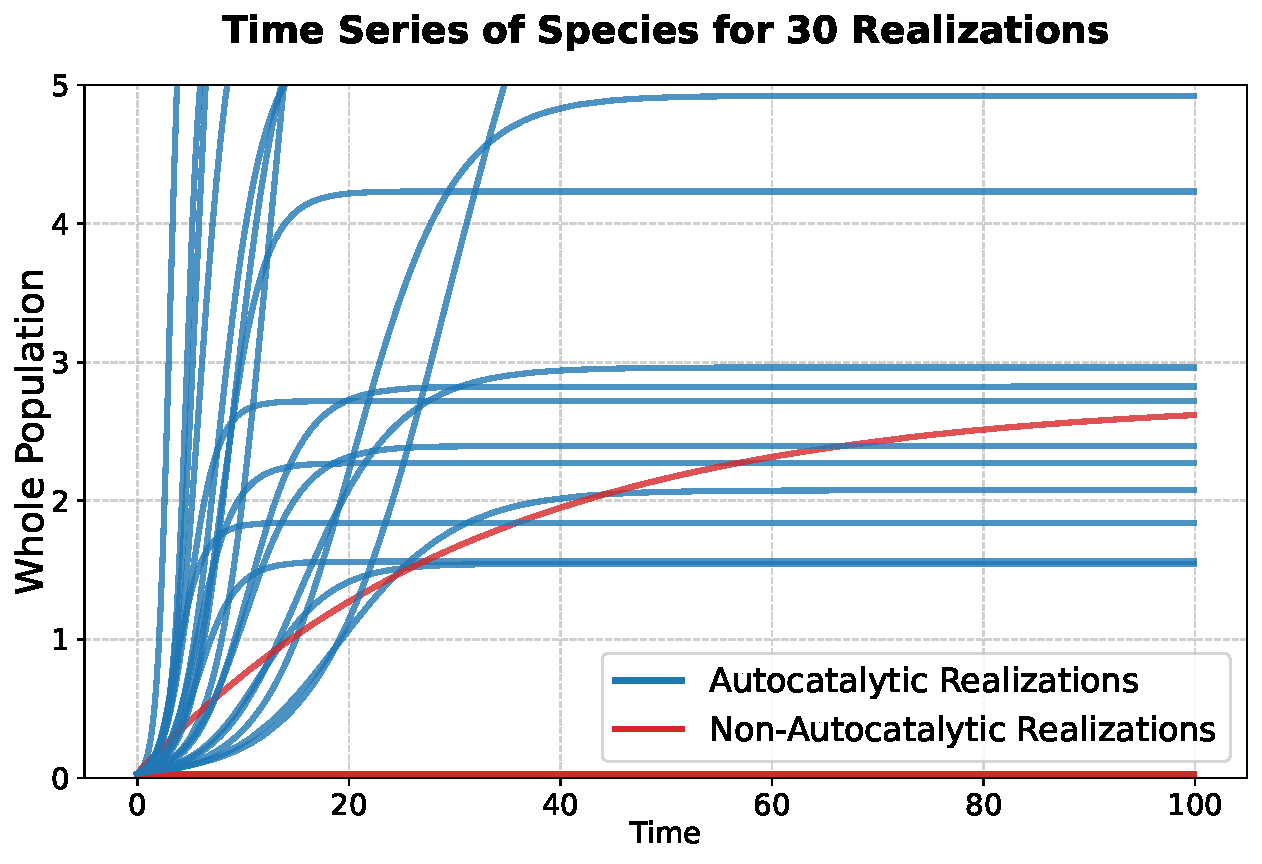
\includegraphics[width=0.45\linewidth]{traj_large_dil_elegant.pdf} 
   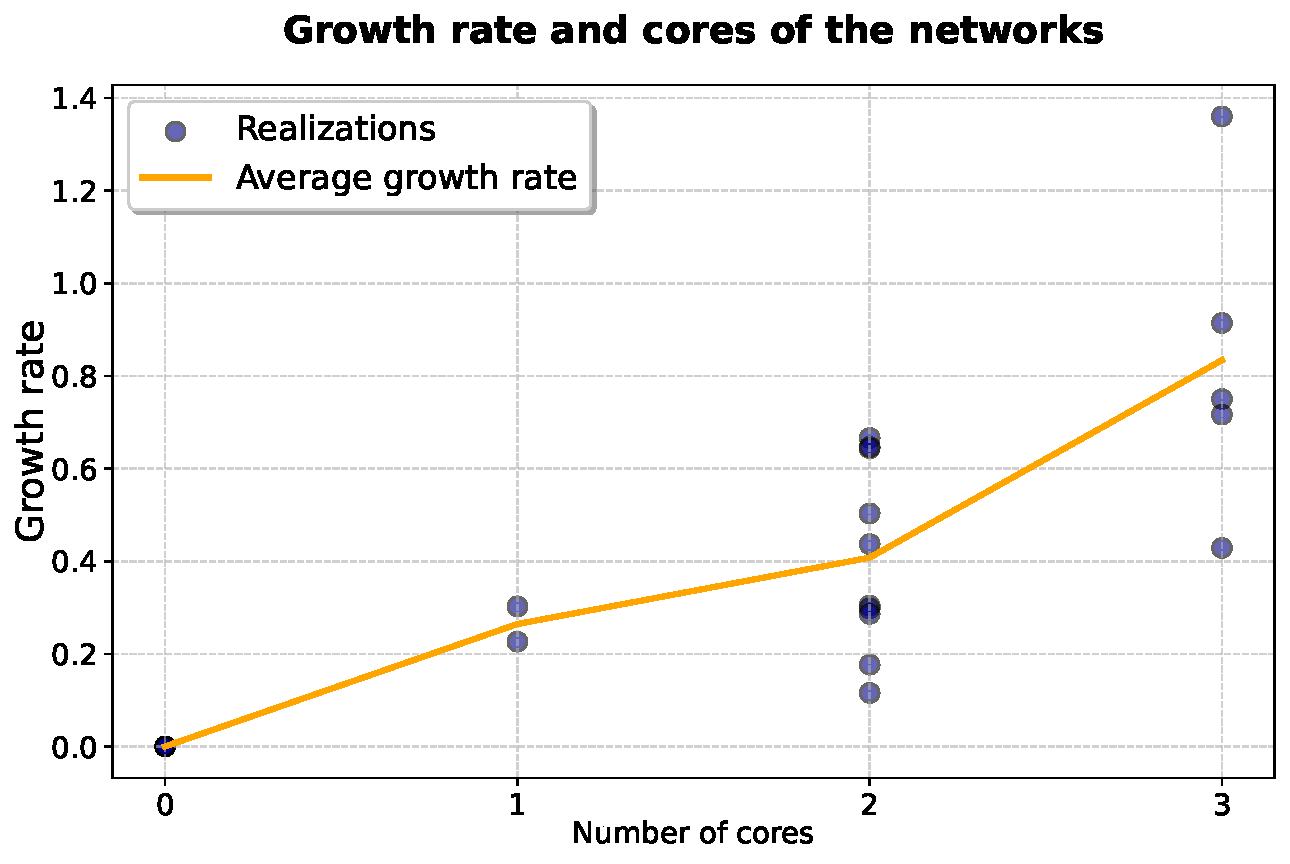
\includegraphics[width=0.45\linewidth]{growth_filtered.pdf} 
   \caption{\small{The simulation is made comparing 30 realizations, over a time of 100.0, considering 3 invaders species and 4 possible reactions. Left plot: systems that show stoichiometric autocatalysis (blue) show also dynamical autocatalysis at small times, systems that don't show stoichiometric autocatalysis (red) either don't grow or grow (hence survive) logarithmically. Right plot: the average growth rate of the network at small times shows positive correlation with the number of cores present in it.}}
    \label{Fig. 1}
\end{figure}

In the left plot of Fig. \ref{Fig. 1}, the blue trajectories represent the evolution of stoichiometrically autocatalytic networks, whereas the red ones don't have this property. Survival means going beyond a certain threshold represented with the dashed horizontal line for these trajectories. Right plot represents the number of cores identified during the realizations and the respective growth rate that those network had. As expected, for stronger autocatalysis (higher number of cores) one expects an average higher growth rate at short times. The surviving non-autocatalytic trajectories seem to follow non-exponential behavior, whereas the surviving autocatalytic ones are all exponential. What seems to happen is that when \textbf{stoichiometric autocatalysis} is present, the network shows \textbf{dynamical autocatalysis} as well, as we wanted to check. 

\\
What is important to notice is that, whenever a non-autocatalytic system still manages to grow, not only it doesn't obviously grow exponentially, but it does following a logarithmic-like behavior (or at least, with a down convexity). We'll see that this behavior is typical only of non-diluted and non-autocatalytic networks.

One important thing that we notice, is that every autocatalytic system will reach a non-equilibrium steady state, under these conditions. Zooming out on the 30 realizations time series, we clearly see that a steady state is reached at not long times:

\begin{figure}[H]
    \centering
    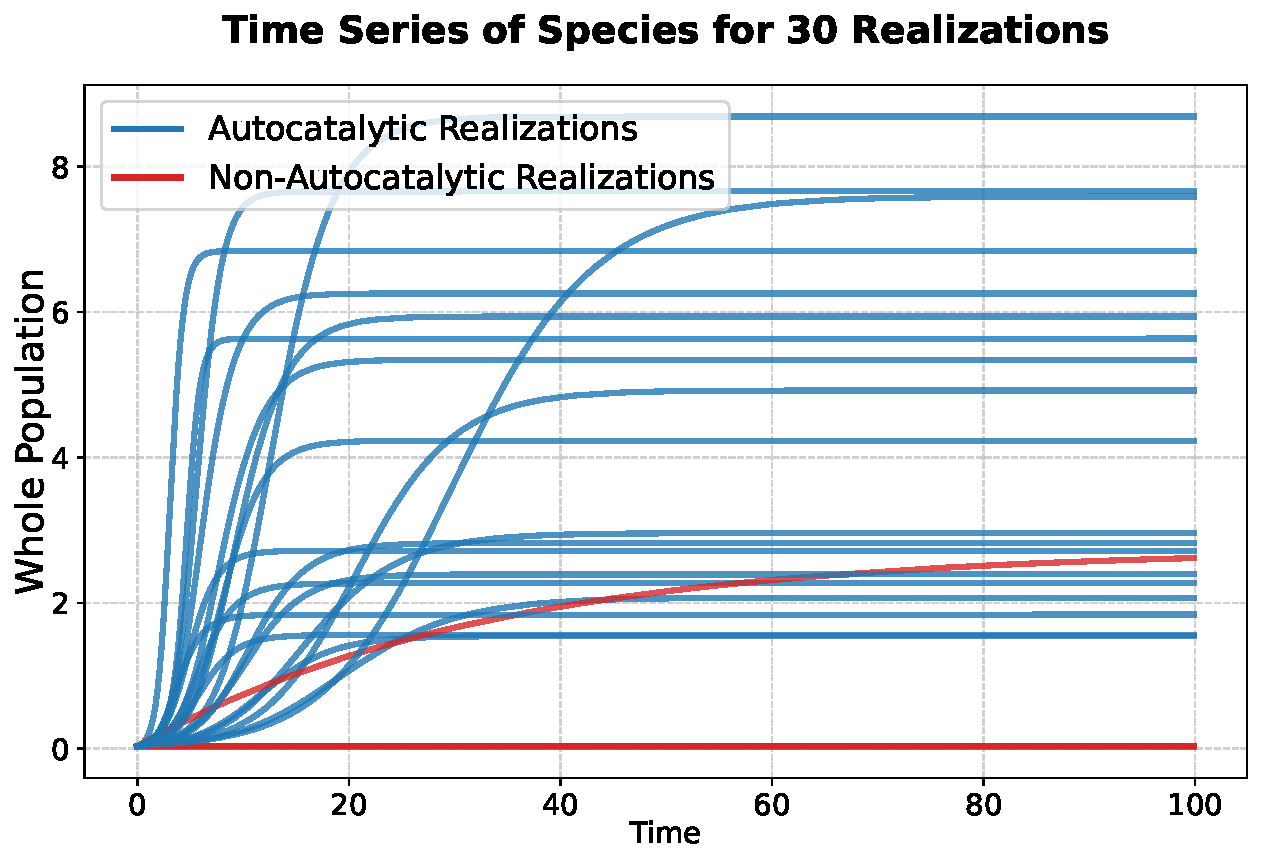
\includegraphics[width=0.7\linewidth]{traj_elegant.pdf} 
    \caption{\small{The simulation is made comparing 30 realizations, over a time of 100.0, considering 3 invaders species and 4 possible reactions. The plot underlines the behavior of the autocatalytic networks (blue) at long time: all of them, in a non-diluted system, reach a stable steady state.}}
    \label{Fig. A}
\end{figure}


When we assume non-diluted, autonomous, non-ambiguous system: \textbf{a non-equilibrium steady state different from zero is reached by every autocatalytic network with MAL; moreover, the evolution towards it follows an exponential growth at small time: the system shows dynamical autocatalysis}.

\subsection{Autonomous non-ambiguous system with MM}
\\ \\
One could now be interested instead in noticing the change for realizations following Michaelis-Menten kinetics instead of MAL. What one could observe in this case is that, often, concentrations may reach an higher value and probably don't even set to a stable fixed point:

\begin{figure}[H]
    \centering
    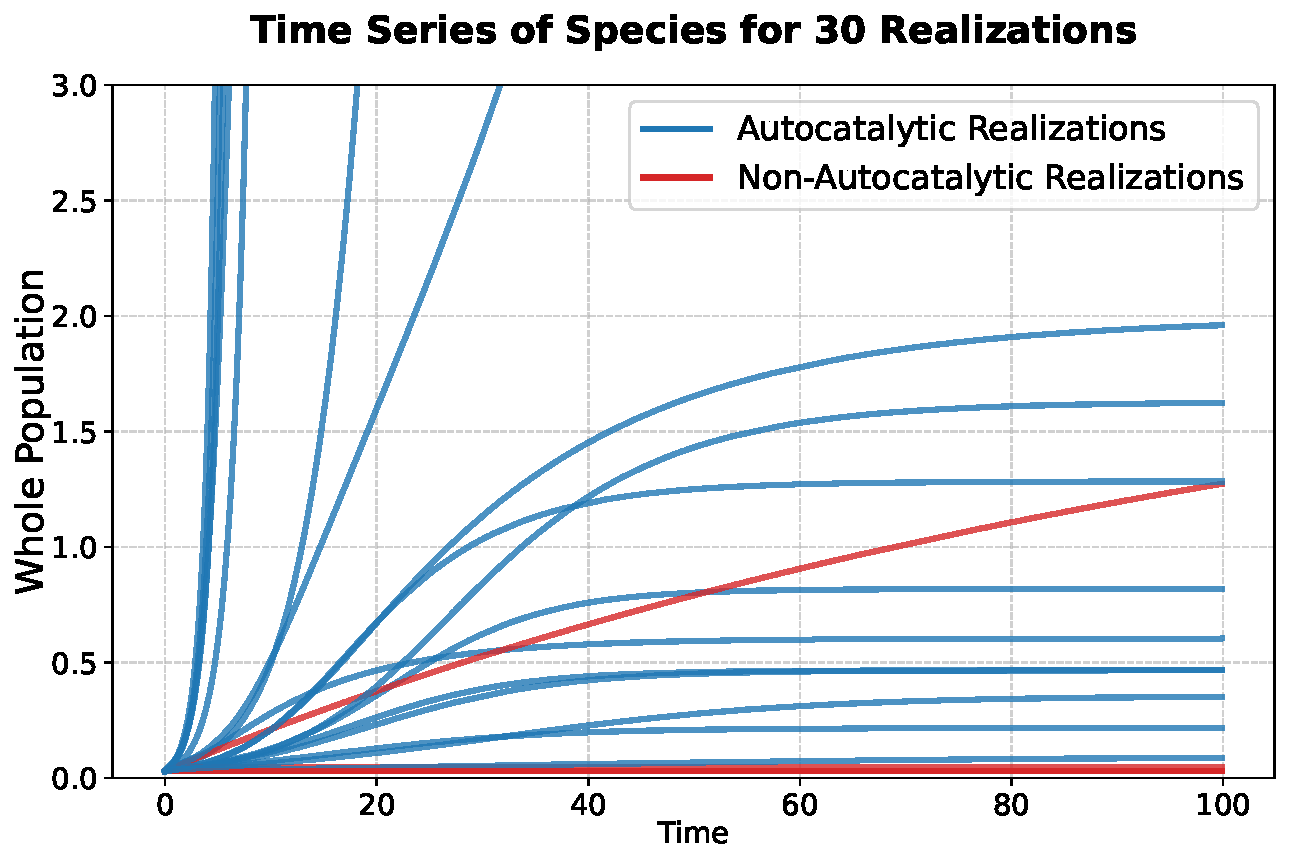
\includegraphics[width=0.6\linewidth]{traj_elegant_MM.pdf} 
 \caption{\small{The simulation is made comparing 30 realizations, over a time of 100.0, considering 3 invaders species and 4 possible reactions.}}
   
    \label{Fig. 2a}
\end{figure}

Zooming in, one would see that the only non-autocatalytic but growing realizations, are doing that more slowly than with linearity. Zooming out instead, we notice that for some choice of the random rates, with MM (a parameter rich kinetic), the systems show instability of the steady state, having unstable-positive feedback cores, as stated in \cite{1}.

\begin{figure}[H]
    \centering
    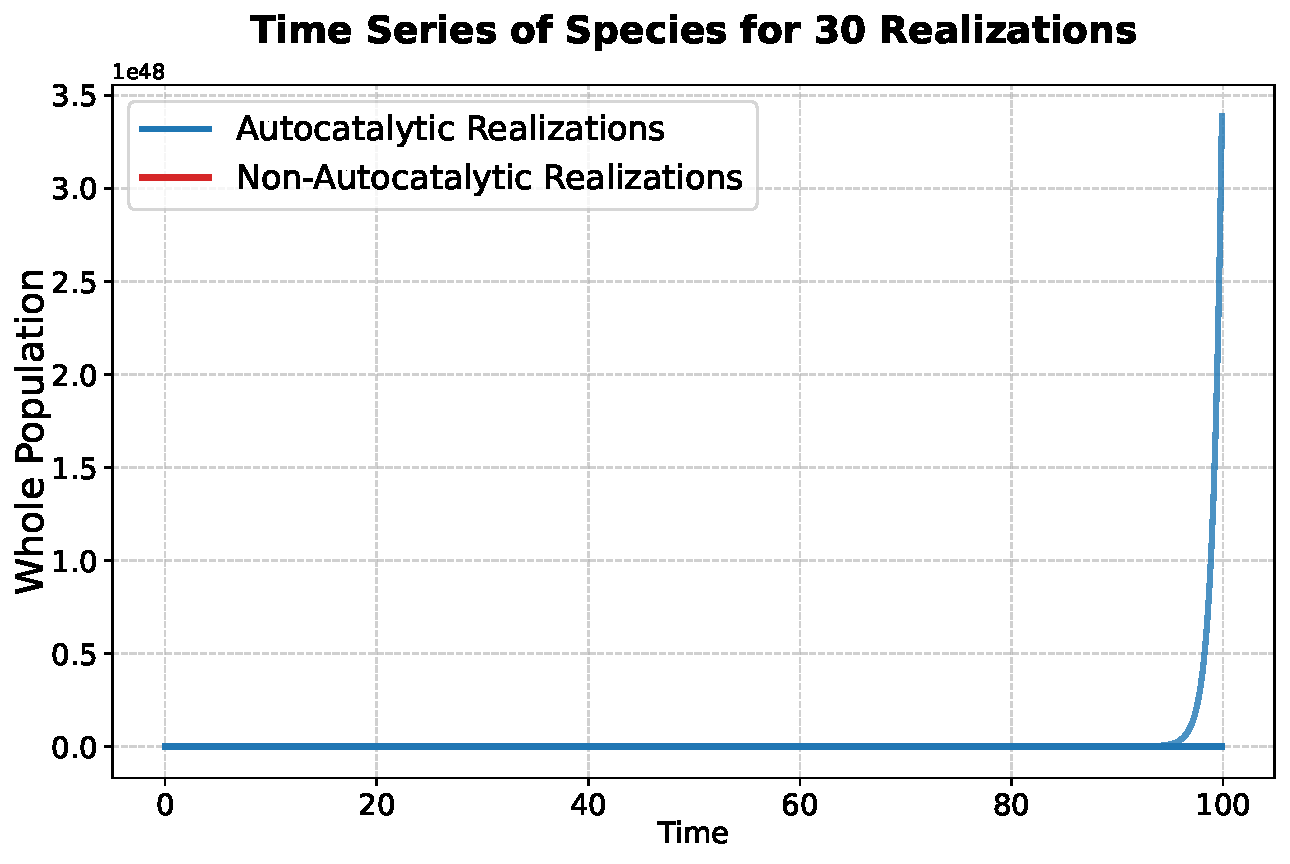
\includegraphics[width=0.6\linewidth]{traj_elegant_MM_.pdf} 
 \caption{\small{The simulation is made comparing 30 realizations, over a time of 100.0, considering 3 invaders species and 4 possible reactions. The behavior of the trajectories resemble the ones using MAL. Higher values of steady state, qualitatively, are reached but sometimes, there is no stable steady state instead.}}
   
    \label{Fig. 2b}
\end{figure}

\subsection{Diluted, autonomous, non-ambiguous system with MAL}
The third case which we may be interested in, is when the system gets diluted, i.e.:

\begin{itemize}
    \item ask for dilution (dilution == True)
    \item ask for autonomy  (autonomy == True)
    \item ask for non-ambiguity (ambiguity == False)
\end{itemize}

As rate law, we used \textbf{mass action law}. This lead to the following $30$ realizations:\\

\begin{figure}[H]
    \centering
    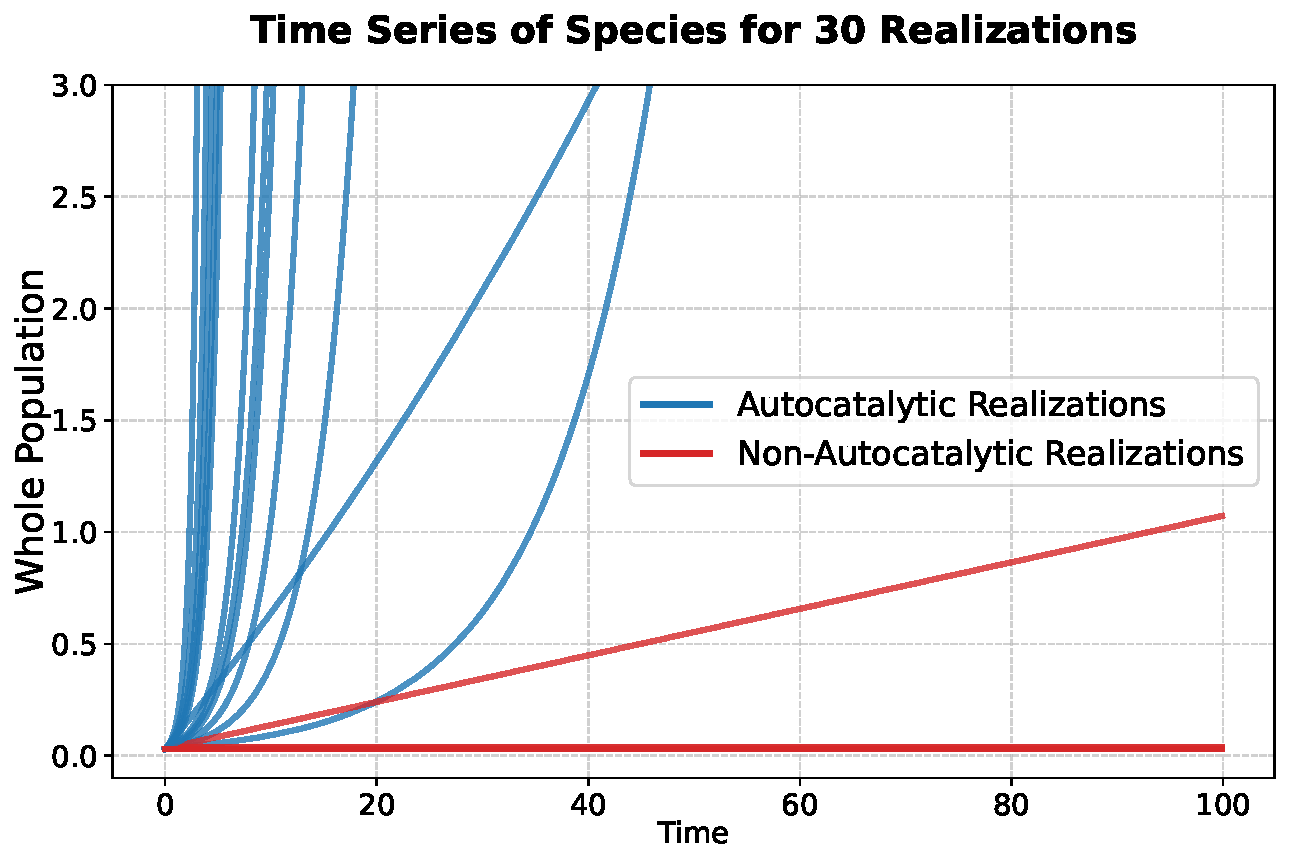
\includegraphics[width=0.45\linewidth]{traj_dil_elegant.pdf} 
   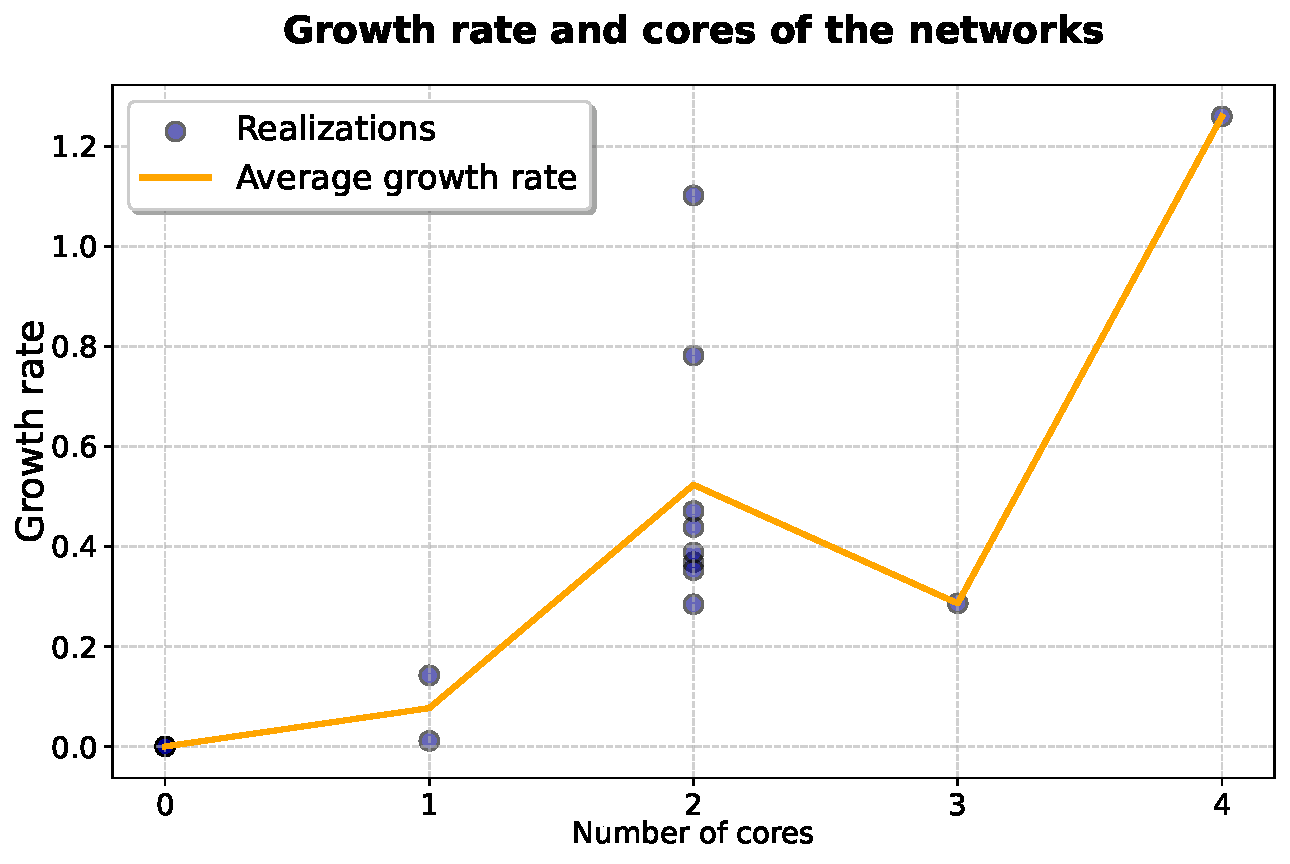
\includegraphics[width=0.45\linewidth]{growth_dil.pdf} 
 \caption{\small{The simulation is made comparing 30 realizations, over a time of 100.0, considering 3 invaders species and 4 possible reactions, the system is diluted. Left plot: systems that show stoichiometric autocatalysis (blue) show also dynamical autocatalysis at small times, systems that don't show stoichiometric autocatalysis (red) either don't grow or grow (hence survive) linearly. Moreover, the autocatalytic ones don't reach a stable steady state. Right plot: the average growth rate of the network at small times shows some sort of positive correlation with the number of cores present in it, more realizations should be taken into account.}}
   
    \label{Fig. 3}
\end{figure}

We notice an important and different behavior in these trajectories: \textbf{stoiochiometric autocatalytic systems continue to be dynamically autocatalytic, given their exponential growth, but in a diluted system, the few non-autocatalytic realizations that survive grow linearly, not anymore "logarithmically"}.
\\

Moreover, we notice that the autocatalytic systems \textbf{don't reach a stable steady state}, as proven in \cite{2}, a priori from the fixed point. 
\\
\\
So \textbf{a diluted system, when it shows stoichiometric autocatalysis, grows indefinetely and exponentially, without ever reaching a steady state}. This is coeherent with the results on dyamical autocatalysis in diluted systems proven in \cite{2}. \textbf{Why instead, non-diluted systems seem to always show a stable steady state? Under what conditions do we reach a Metlzer-shaped Jacobian?} In the following, we show the comparison between 15 realizations for a non-diluted and a diluted one:

\begin{figure}[H]
    \centering
    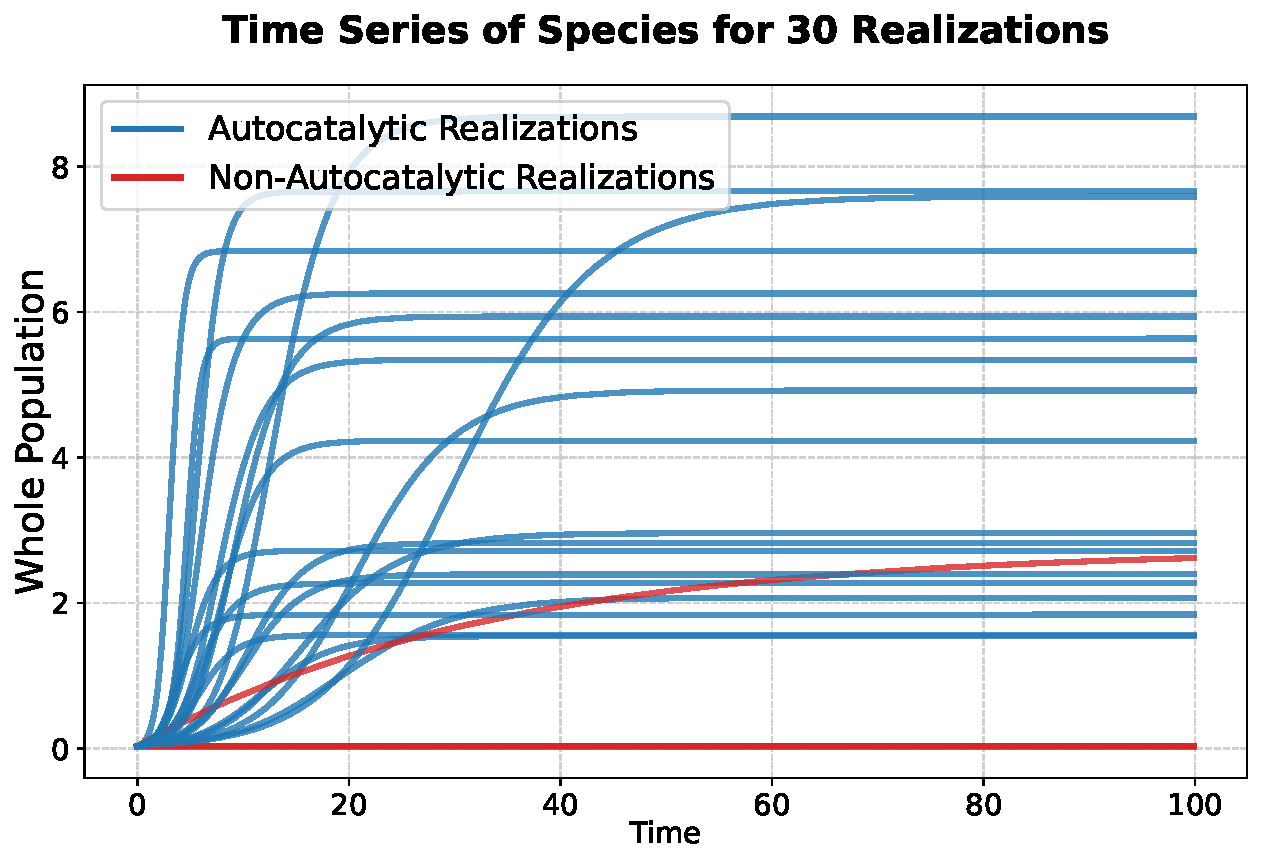
\includegraphics[width=0.45\linewidth]{traj_elegant.pdf} 
   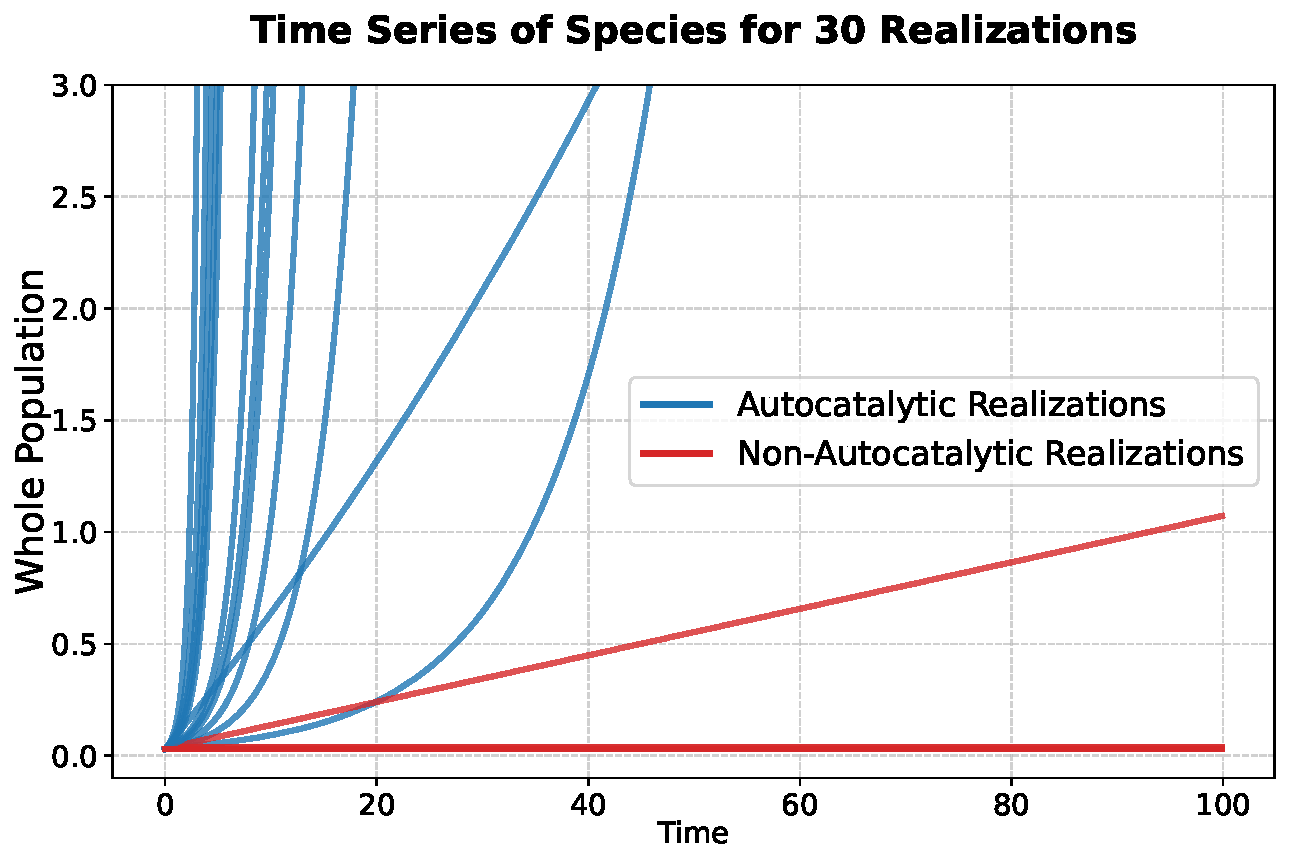
\includegraphics[width=0.45\linewidth]{traj_dil_elegant.pdf} 
 \caption{\small{The simulation is made comparing 30 realizations, over a time of 100.0, considering 3 invaders species and 4 possible reactions. Left plot shows a non-diluted system, whereas the right one shows a diluted one. Systems that show stoichiometric autocatalysis (blue) show also dynamical autocatalysis at small times, systems that don't show stoichiometric autocatalysis (red) either don't grow or grow (hence survive) but with a different behavior whether the system is diluted or not.}}
   
    \label{Fig. B}
\end{figure}

\begin{itemize}
    \item Non-diluted systems show stable steady states for autocatalytic realizations and convex growth for some non-autocatalytic ones (left plot)
    \item Diluted systems don't show stability of steady states for autocatalytic realizations but show linear growth for some non-autocatalytic ones (right plot)
\end{itemize}



\subsection{Autonomous ambiguous system with MAL}
\\
Going back to a non-diluted network, we can remove the ambiguity assumption: a property that will not influence stoichiometry, hence the autocatalytic features, but will instead influence directly the dynamics of the systems.

\begin{comment}
We set:

\begin{itemize}
    \item ask for no dilution (dilution == False)
    \item ask for autonomy  (autonomy == True)
    \item allow ambiguity (ambiguity == True)
    \item MAL
\end{itemize}

\begin{flushleft}
    Running 20 different realizations, we end up with:
\end{flushleft}

\begin{figure}[H]
    \centering
    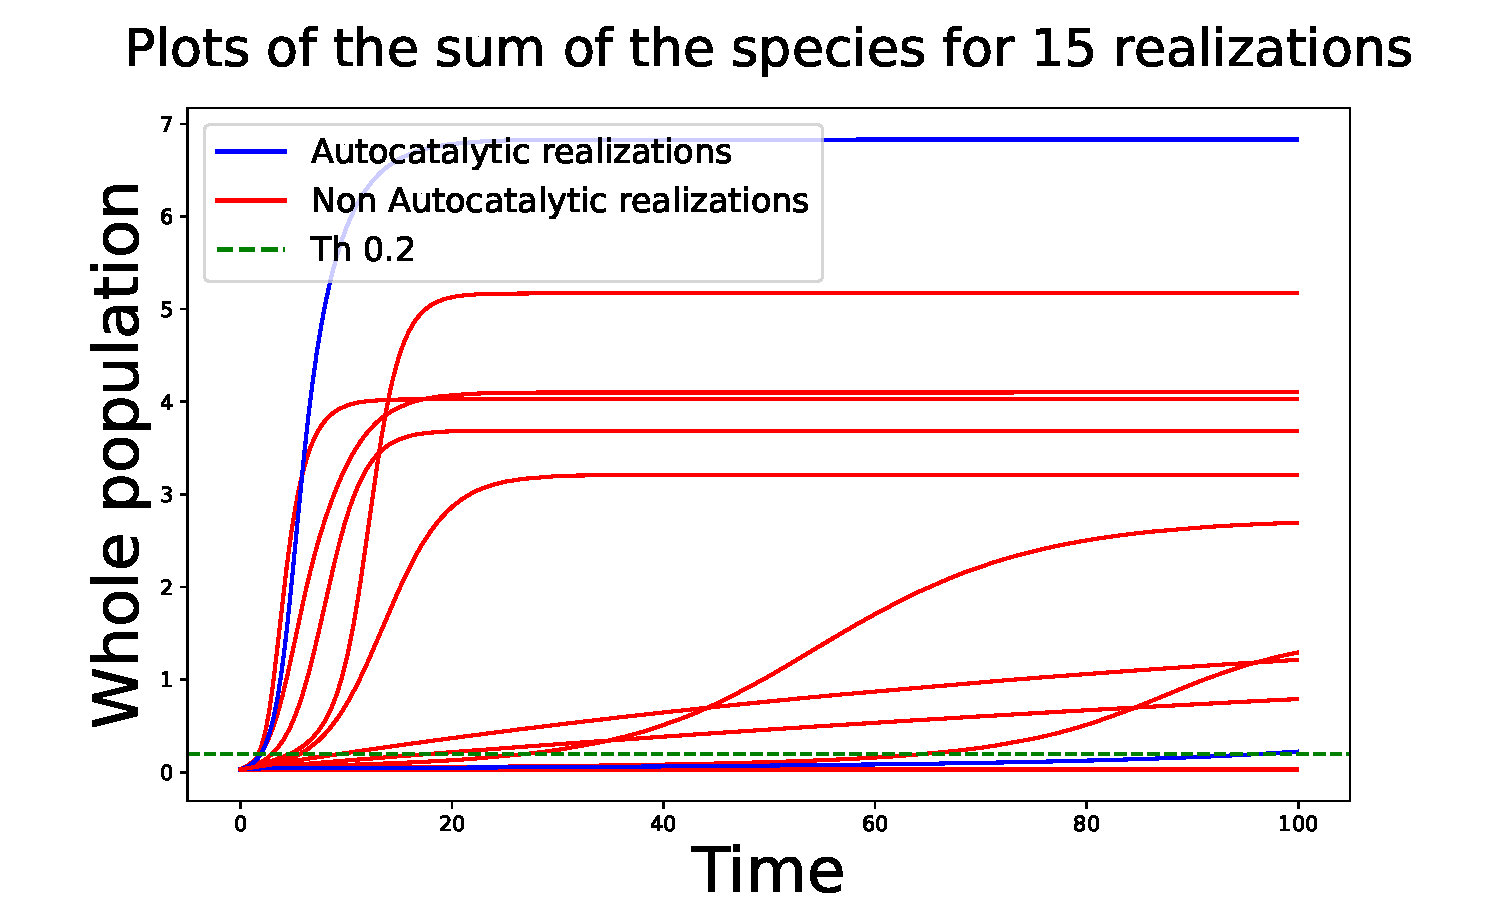
\includegraphics[width=0.6\linewidth]{traj_amb.pdf} 
 \caption{\small{The simulation is made comparing 15 realizations, over a time of 100.0, considering 3 invaders species and 4 possible reactions. Systems that show stoichiometric autocatalysis (blue) show also dynamical autocatalysis at small times, but the same can happen for non autocatalytic ones (red) as a result of the allowed ambiguity.}}
    \label{Fig. 4}
\end{figure}

Showing that, allowing ambiguity, autocatalysis is not affected by the change in feasible reactions, but dynamically it will be more likely to show instability: the non-autocatalytic networks can still present exponential growth.

\end{comment}
Indeed \textbf{catalysis} may still be present, thanks to the allowed ambiguity, but the stoichiometric matrix would obviously not be affected by it: it will not identify cores that instead may be present. This is why many non-autocatalytic realizations still present dynamical autocatalysis: they also show stoichiometric catalysis or autocatalysis, but the stoichiometric matrix is not able to see it.


\subsection{Non-autonomous non-ambiguous system with MAL}
\\
We are now interested instead in the system to be non-autonomous, so it might be possible for reactions to show explicit degradation.

\begin{comment}

\begin{itemize}
    \item ask for no dilution (dilution == False)
    \item ask for no autonomy  (autonomy == False)
    \item ask for non-ambiguity (ambiguity == False)
    \item MAL
\end{itemize}

\begin{flushleft}
    Running 20 different realizations, we end up with:
\end{flushleft}

\begin{figure}[H]
    \centering
    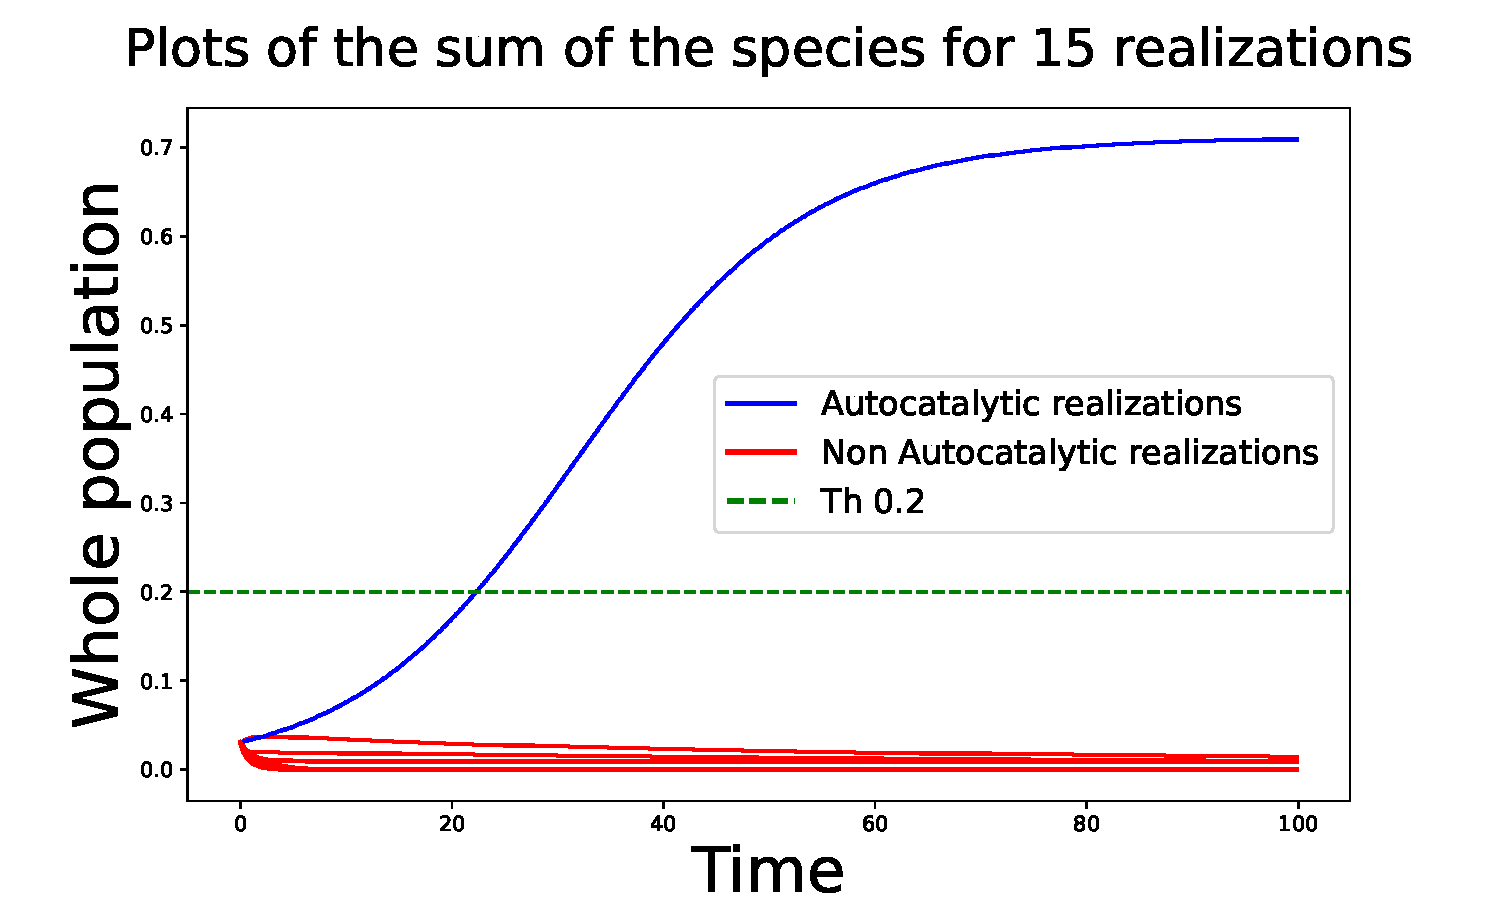
\includegraphics[width=0.5\linewidth]{traj_aut.pdf} 
   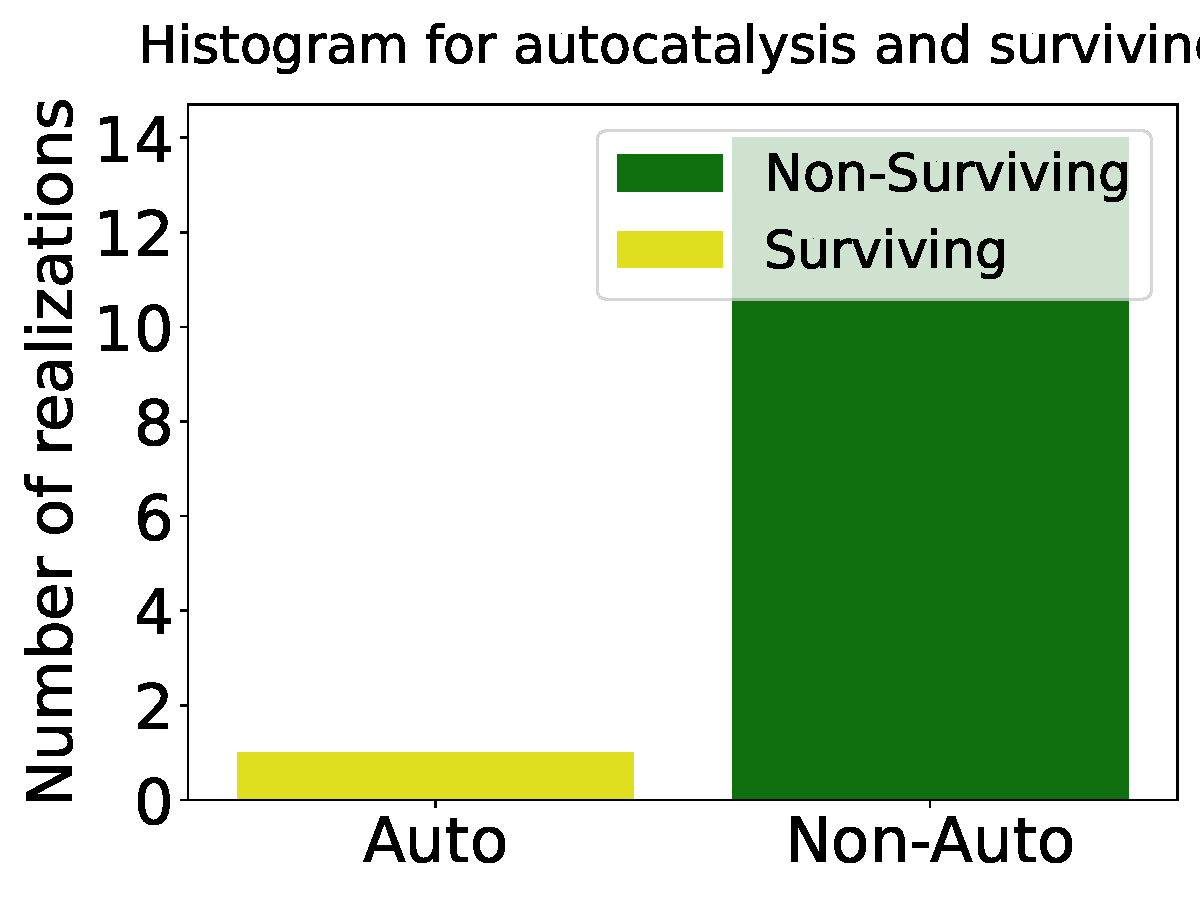
\includegraphics[width=0.4\linewidth]{confusion_matrix_aut.pdf} 

    \caption{\small{The simulation is made comparing 15 realizations, over a time of 100.0, considering 3 invaders species and 4 possible reactions. Left plot: systems that show stoichiometric autocatalysis (blue) show also dynamical autocatalysis at small times, systems that don't show stoichiometric autocatalysis (red) don't grow at all or get completely degraded. Right plot: the few stoichiometric network are the only one that manage to overcome the threshold and survive.}}
    \label{Fig. 5}
\end{figure}

\begin{flushleft}
We notice that,

\end{comment}
Allowing non-autonomy, we're allowing direct degradation to be present in the system: as a result, autocatalytic networks become more rare and when they appear they grow to much smaller steady states, whereas non autocatalytic ones embedded with also degradation reactions, reach \textbf{zero} concentration steady state already at small times: the population disappears.
%\end{flushleft}

\subsection{Larger networks}
We can now try to add an higher number of species and reactions, using
$ttot = 100.0, dt = 10^{-3}, REALIZATIONS = 15, N_X = 10, N_Y = 5, N_{RY} = 10.$


\begin{flushleft}
And considering:    
\end{flushleft}
\begin{itemize}
    \item No dilution
    \item Autonomy
    \item Non-ambiguity
    \item Mass Action Law
\end{itemize}

\begin{flushleft}
    Resulting in 
\end{flushleft}

\begin{figure}[H]
    \centering
    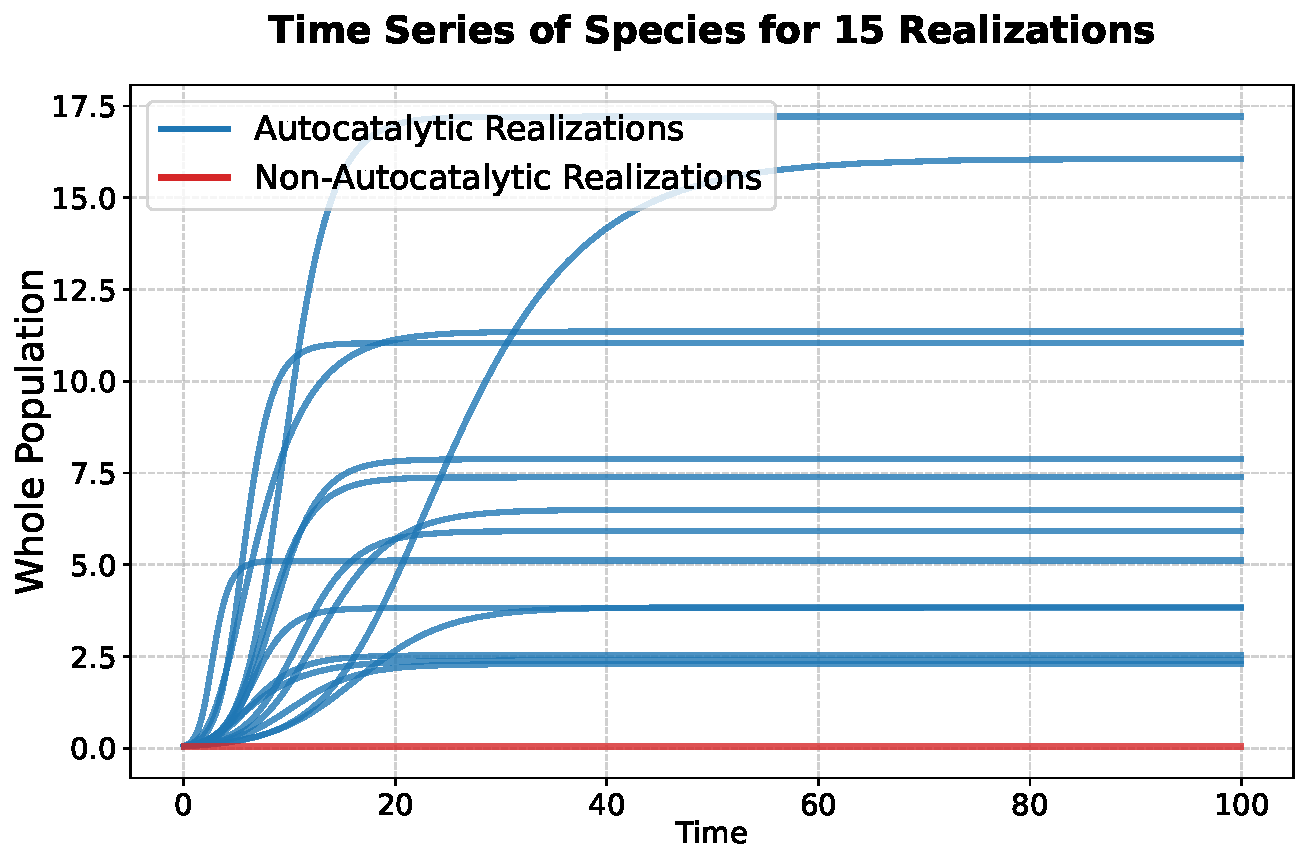
\includegraphics[width=0.6\linewidth]{traj_large_elegant.pdf} 
    \caption{\small{The simulation is made comparing 15 realizations, over a time of 100.0, considering 5 invaders species and 10 possible reactions. Systems that show stoichiometric autocatalysis (blue) show also dynamical autocatalysis at small times.}}
    \label{Fig. 6}
\end{figure}

As expected, more species and reactions help autocatalysis to show up. In fact, $13/15$ realizations showed the existence of cores, bringing an exponential growth to all of them.

A large \textbf{diluted} network instead, with the others parameters being kept the same, will show the same behaviour, always having a \textbf{linear} growth for the few surviving non-autocatalytic (the plot is zoomed in on the $y$ axis):

\begin{figure}[H]
    \centering
    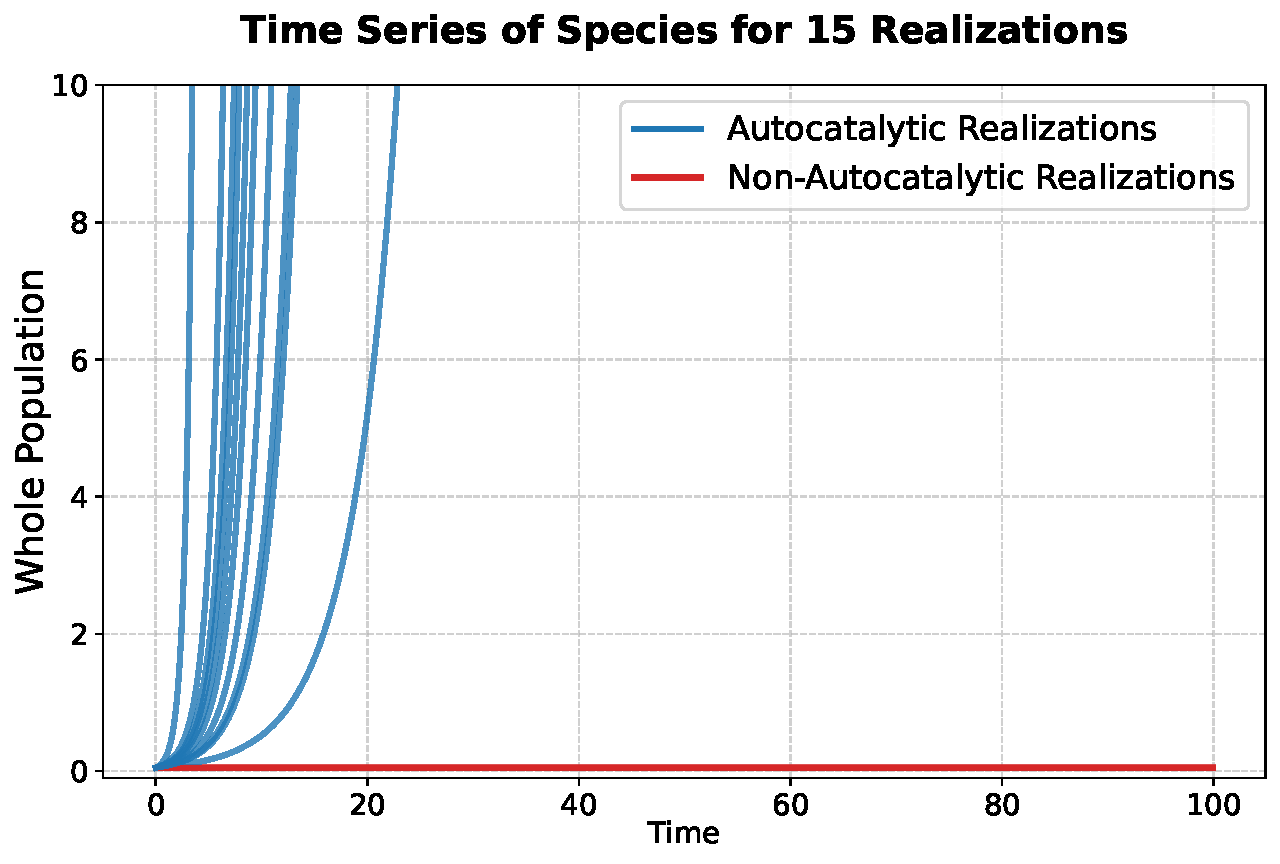
\includegraphics[width=0.6\linewidth]{traj_large_elegant_dil.pdf}
       \caption{\small{The simulation is made comparing 15 realizations, over a time of 100.0, considering 5 invaders species and 10 possible reactions. Systems that show stoichiometric autocatalysis (blue) show also dynamical autocatalysis at small times, exploding away from a steady state. Some non-autocatalytic realizations (red) still manage to grow linearly. }}
    \label{Fig. 7}
\end{figure}

\section{Particular cases}

\subsection{Overall conservation laws in autocatalytic networks}

Note that not always an autocatalytic realization manages to grow exponentially at small times: an interesting scenario that may happen, is when the random generation of the stoichiometric matrix produces a non-full rank matrix, that still presents some cores. In this case, if a specific conservation law for the system appears (one that limits a linear combination of the all the species in the network), the overall population will not be able to grow. A conservation law $\Vec{l}$ is such that

\begin{center}
\begin{equation}
    \Vec{l}S_P = \Vec{0}
\end{equation}
\end{center}

An example of this is the following autocatalytic network which presents a core but also a conservation law concerning all the $3$ species, being not a full rank matrix

\begin{center}
    \begin{equation}
        S_P=\begin{pmatrix}
            1 & -1 & 0 & 0 & -1 & -1 \\
            0 & 0 & -1 & 1 & 1 & -1 \\
            -2 & 2 & 1 & -1 & 1 & -1 \\
        \end{pmatrix}
    \end{equation}
\end{center}

In such a case, the exponential growth of the overall sum of the species, which would be dynamically guaranteed by the presence of a core, is instead limited by the conservation law, which imposes:

\begin{center}
    \begin{equation}
        2\textrm{y}_1+\textrm{y}_2+\textrm{y}_3=const
    \end{equation}
\end{center}

Therefore, in such systems, dynamical autocatalysis will not show up, being limited by the conservation law of the system. Even though the system shows autocatalytic cores, the conservation law present in the whole network will limit the grow of the total sum of the population.
Obviously, this extends to non-autocatalytic networks: whenever a linear combination with positive coefficients for all the species in the network appears, the sum of the species will be upper bounded by a value that will limit its growth. 

\subsection{Partial conservation laws in non-autocatalytic networks}
We' ve seen in figure \ref{Fig. 5} that, in a diluted system, non-autocatalytic realizations either don't grow when a conservation law concerns all the species in the network, or they can survive and grow linearly. Let's take the non-autocatalytic network that survived in figure \ref{Fig. 5}:

\begin{center}
    \begin{equation}
        S_P=\begin{pmatrix}
            -1 & 1 & 1 & -1 & 1 & -1 \\
            1 & -1 & -1 & 1 & -1 & 1 \\
            0 & 0 & 1 & 0 & 0 & 1 \\
        \end{pmatrix}
    \end{equation}
\end{center}

This network doesn't have any core, but it has a conservation law

\begin{center}
    \begin{equation}
        \Vec{l}=\begin{pmatrix}
            1 \\
            1 \\
            0 \\
        \end{pmatrix}
         \quad \implies \quad l \coloneqq \textrm{y}_1+\textrm{y}_2=constant
    \end{equation}
\end{center}

and since the rank of $S_P$ isn't maximum, we'll have only 2 independent dynamical equations and 1 constraint. Using MAL:

\begin{center}
    \begin{equation}
    \begin{aligned}
    \textrm{y}_1 &= l -\textrm{y}_2 \\
        \frac{d \textrm{y}_2}{d t} &=j_1-j_2-j_3+j_4-j_5+j_6 =\\
        &=\left(k_1+k_4+k_6\right) \textrm{y}_1- \left(k_2+k_3+k_5 \right) \textrm{y}_2\\
        \frac{d \textrm{y}_3}{d t} &= j_3+j_6 = k_3 \textrm{y}_2 + k_6 \textrm{y}_1 
        \end{aligned}
    \end{equation}
\end{center}

Inserting the first equation in the others we remove $\textrm{y}_1$

\begin{center}
    \begin{equation}
    \begin{aligned}
        \frac{d \textrm{y}_2}{d t} &=-\left( \sum^6_i k_i\right) \textrm{y}_2 + \left( k_1+k_4+k_6\right) l\\
        \frac{d \textrm{y}_3}{d t} &= \left(k_3 - k_6 \right) \textrm{y}_2 + k_6 l
        \end{aligned}
        \label{12}
    \end{equation}
\end{center}

For simplicity of notation, we' ll call $\textrm{K} \coloneqq \sum^6_i k_i $ and $\textrm{y}^0_i = \textrm{y}_i(t=0)$.
The first equation can now be solved on its own, leading to 

\begin{center}
    \begin{equation}
        \textrm{y}_2 (t) = \frac{l}{K} + \left(\textrm{y}^0_2 - \frac{l}{K} \right) e^{-Kt}
        \end{equation}
        \label{13}
\end{center}

which can now be inserted in the second equation of \eqref{12}, leading to an analytically solvable equation for $\textrm{y}_3 (t)$

\begin{center}
    \begin{equation}
    \begin{aligned}
        \frac{d \textrm{y}_3}{d t} &= \left(k_3 - k_6 \right) \left[ \frac{l}{K} + \left(\textrm{y}^0_2 - \frac{l}{K} \right) e^{-Kt}\right] + k_6 l
        \end{aligned}
        \label{14}
    \end{equation}
\end{center}

Now, we remind that 

\begin{center}
    \begin{equation}
        \frac{d \textrm{y}_{tot}}{d t} = \frac{d \textrm{y}_3}{d t} = \left(k_3 - k_6 \right) \left[ \frac{l}{K} + \left(\textrm{y}^0_2 - \frac{l}{K} \right) e^{-Kt}\right] + k_6 l
    \end{equation}
\end{center}

This shows that, after very few steps, $\textrm{y}_{tot}$ will grow linearly in time due to the presence of the 2-species conservation law. Indeed, solving \eqref{14}

\begin{center}
    \begin{equation}
        \textrm{y}_3 (t) = l \left(\frac{k_3 - k_6}{K} + k_6\right) t + \frac{k_6-k_3}{K}\left(\textrm{y}^0_2 - \frac{l}{K} \right) e^{-Kt} + const
    \end{equation}
\end{center}

and 

\begin{center}
    \begin{equation*}
        \textrm{y}_{tot} (t) = y^0_1 + y^0_2 + l \left(\frac{k_3 - k_6}{K} + k_6\right) t + \frac{k_6-k_3}{K}\left(\textrm{y}^0_2 - \frac{l}{K} \right) e^{-Kt} + const
    \end{equation}
\end{center}


\begin{center}
    \begin{equation*}
        \textrm{y}_{tot} (t) \sim l\left(\frac{k_{-1} - k_{-3}}{K} + k_{-3}\right) t
    \end{equation}
\end{center}

\section{Successive invasions}

In this section we will analyze the concept of "community" and "evolution". What happens when a set of invaders come in to destabilize the equilibrium of a community of species? Can they "invade" the original community thanks to autocatalysis? Will they survive or will they die, and how is this related to the introduction of autocatalytic cores?

\subsection{Random Matrices and Simulation Setup}
The idea is to start from a well defined number of food species $N_F$ in a certain "environment". The food set will have a constant value chosen randomly from a uniform distribution, and they will mantain the network out of equilibrium,

The next step is to define the properties of the invaders. Each $ttot$ a new set of $N_Y$ invaders will be added to the network, through a set of $N_{RY}$ reversible reactions and an initial concentration taken randomly (from a uniform distribution). Here we assume to have \textbf{autonomous, non-ambiguous and non-diluted} systems. Hence, the new $Y$'s can either evolve by themselves or exploiting the food species $F$ or the original species $X$. The former are constants, the latter are instead not present at the beginning. Depending whether the invaders are considered \textbf{competing} species against the $X$'s or \textbf{parasites}, different types o reactions can be allowed:

\begin{itemize}
    \item \textbf{Competition}: $Y$'s can show autocatalysis on their own

\begin{equation}
		\begin{split}
\ce{\textsf{Y}_i & <--> \textsf{Y}_j } \quad \quad i \neq j \\ 
\ce{\textsf{Y}_i & <--> \textsf{Y}_j + \textsf{Y}_k } \quad \quad i \neq j,k \\ 
\ce{\textsf{F}_i + \textsf{Y}_j & <--> \textsf{Y}_k + \textsf{Y}_l } \quad \quad j \neq k,l \\ 
\ce{\textsf{F}_l + \textsf{Y}_i & <--> \textsf{Y}_j + \textsf{F}_m } \quad \quad i \neq j , \ l \neq m\\ 
\end{split} 
\end{equation}
\\

\item \textbf{Parasites}: $Y$'s can reproduce only through $F$'s or $X$'s

\begin{equation}
		\begin{split}
\ce{\textsf{Y}_i & <--> \textsf{Y}_j } \quad \quad i \neq j \\ 
\ce{\textsf{F}_i + \textsf{Y}_j & <--> \textsf{Y}_k + \textsf{Y}_l } \quad \quad j \neq k,l \\ 
\ce{\textsf{F}_l + \textsf{Y}_i & <--> \textsf{Y}_j + \textsf{F}_m } \quad \quad i \neq j , \ l \neq m\\ 
\end{split} 
\end{equation}
\\

\end{itemize}

This means we are randomizing, through the stated constraints, the two matrices $S^-_Y$ and $S^+_Y$, in order to get $S_Y =S^-_Y-S^+_Y  \in Z^{{(N_F+N_Y)} \times N_{RY}}$. We'll call the overall matrix $S=S_Y$ for now.

As before, for thermodynamic consistency, we randomize the vector of the standard chemical potentials $\pmb{\mu}_0$ and of the forward rates $\pmb{k}_+$ such that

\begin{center}
    \begin{equation}
       k_{-i} = k_{+i} e^{\Delta G_0} = e^{S^T\pmb{\mu}_0} \quad \forall i \in 1, . . ., N_{RY}
    \end{equation}
\end{center}


The next step is the measure of autocatalysis in the network: the overall matrix $S$ (with reversed reactions) is given as an input for the cores' searching algorithm. Afterwards, the entire network is dynamically simulated: the first invasion begins.

\begin{figure}[H]
    \centering
    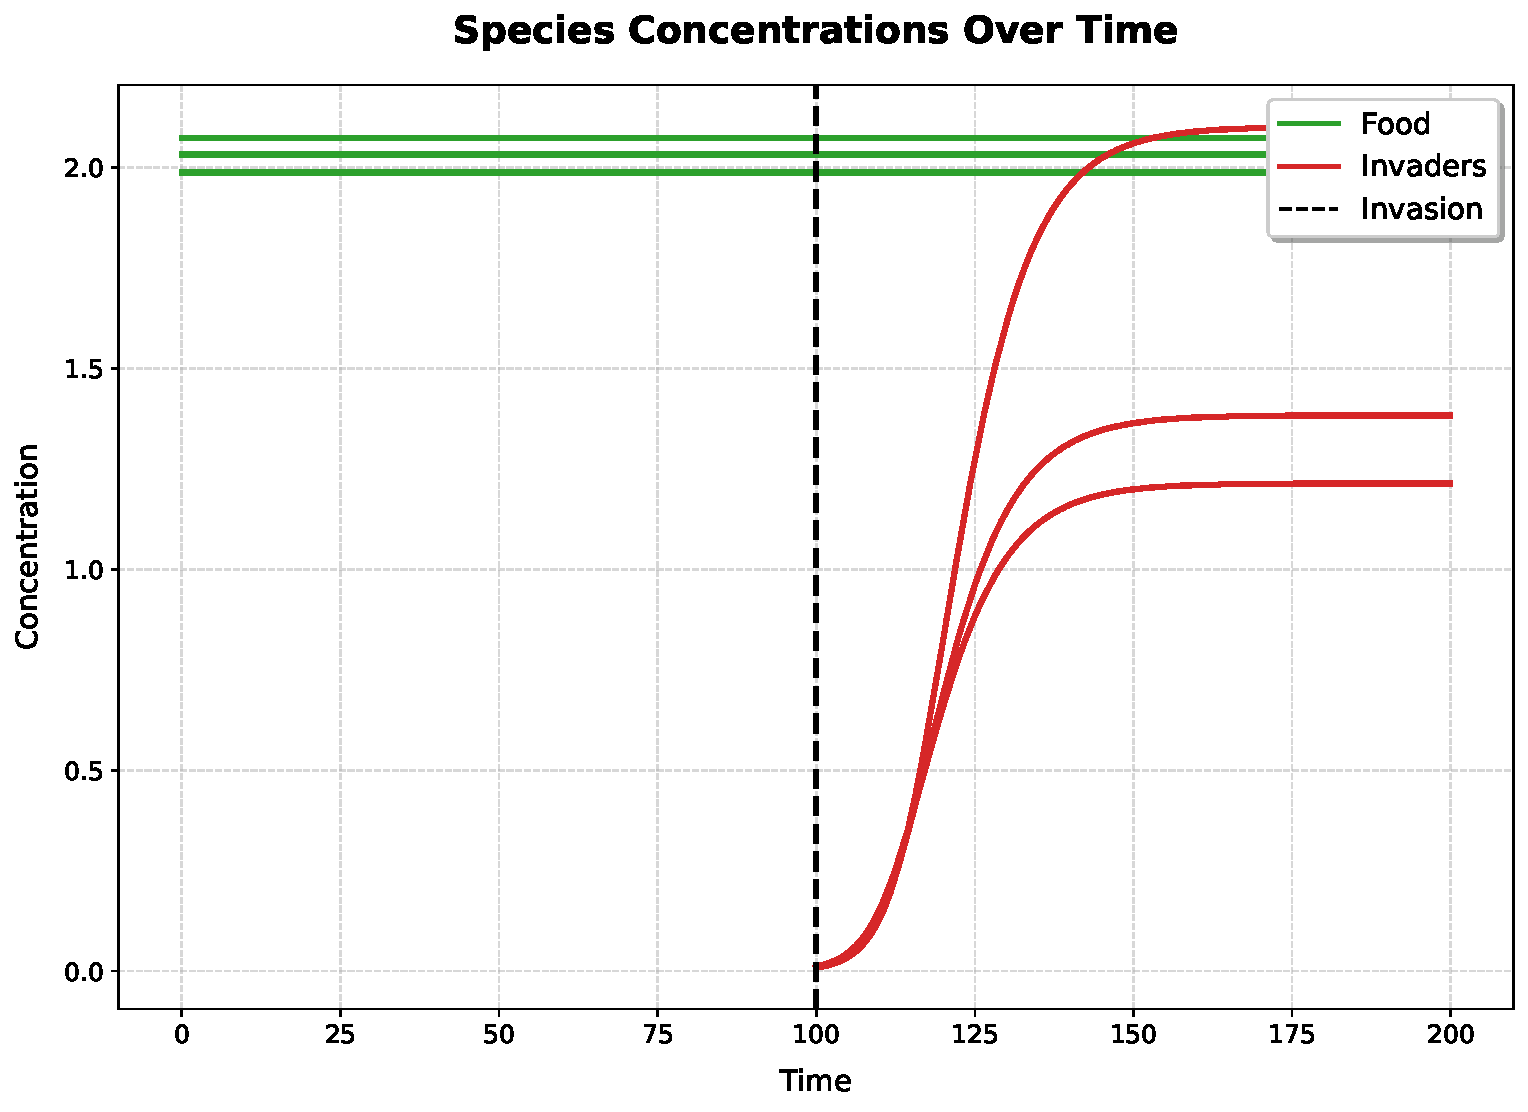
\includegraphics[width=0.6\linewidth]{Successive_species_concentrations.pdf} 
    \caption{\small{Sketch of a single "invasion", the food $N_F=3$ was there until $ttot=100.0$. After that, the first $N_Y=3, \ N_{RY}=3$ arrive and autocatalytically grow}}
    \label{Fig. 8}
\end{figure}

The first set of invaders, can either die (or not grow enough) or grow exponentially thanks to autocatalysis. If the latter happens, after a time $ttot$, the surviving invaders will become original species (called $X$'s), being now allowed to evolve freely but also \textbf{to be exploited and interact} with new set of invaders, that will come afterwards. Indeed, each time $ttot$ it can happen that

\begin{itemize}
    \item \textbf{The set of invaders doesn't survive}
    \begin{itemize}
        \item[-] $N_F$ food species stay constant
        \item[-] The original community remains the same after the interaction with the invaders
        \item[-] A new set of $N_Y$ invaders is introduced
    \end{itemize}
    \item \textbf{The set of invaders survives}
     \begin{itemize}
        \item[-] $N_F$ food species stay constant
        \item[-] The original community is updated, the invaders become part of the original community
        \item[-] A new set of $N_Y$ invaders is introduced
    \end{itemize}
\end{itemize}

We will call $S_X$ the matrix of the original species, i.e. the non-food ones that were already there when new invaders come. $S_X$ will then be the matrix of the previous invaders that managed to survive. After the first invasion, then $S=S_X=S_Y$. The process continues iteratively such that

\begin{itemize}
    \item \textbf{The set of invaders doesn't survive}
    \begin{center}
    $S=S_X$ and $S_Y$ is discarded
    \end{center}
      \item \textbf{The set of invaders survives}   
\begin{center}
\begin{equation}
    S = \begin{pmatrix}
        \begin{pmatrix}
            S_X \\ \\
            \pmb{0}
        \end{pmatrix}, & S_Y
    \end{pmatrix}
\end{equation}
\end{center}
        \end{itemize}


The vectors $\pmb{\mu}_0, \pmb{k}_+, \pmb{k}_-$ will be randomly updated following thermodynamic consistency, depending on whether new species are added to the community or not.

\\




\begin{comment}
As explained before, these original species are allowed to react between each other in every \textbf{non-ambiguous} possible way, as long as they respect the random sampled (between 0 and 2) maximal order for the reactions. This said, the first random matrix we generate, will be $S_X \in Z^{N_X \times N_{RX}}$, through the randomization of $S^-_X$ and $S^+_X$, and it will allow for reactions of any type between $X$'s species.

As before, for thermodynamic consistency, we randomize the vector of the standard chemical potentials $\pmb{\mu}_0$ and of the forward rates $\pmb{k}_+$ such that

\begin{center}
    \begin{equation}
       k_{-i} = k_{+i} e^{\Delta G_0} = e^{S^T\pmb{\mu}_0} \quad \forall i \in 1, . . ., N_R
    \end{equation}
\end{center}

Once the stoichiometry and the kinetics for the first $N_{RX}$ reactions is defined, these first $N_{X}$ species will be kept constant during all the process to guarantee these and the next reactions to be mantained out of equilibrium. We can therefore consider these first species as "food" for all the new incoming ones.
The next step is to define the properties of the invaders. Each $ttot$ a new set of $N_Y$ invaders will be added to the networks, through a set of $N_{RY}$ reversible reactions. Here we assume to have \textbf{autonomous, non-ambiguous and non-diluted} systems. Hence, the new $Y$'s can either evolve by themselves or exploiting the food species $X$ which, at least for the first invasion, are constants:

\begin{equation}
		\begin{split}
\ce{\textsf{Y}_i & <--> \textsf{Y}_j } \quad \quad i \neq j \\ 
\ce{\textsf{Y}_i & <--> \textsf{Y}_j + \textsf{Y}_k } \quad \quad i \neq j,k \\ 
\ce{\textsf{Y}_i + \textsf{Y}_j & <--> \textsf{Y}_k + \textsf{Y}_l } \quad \quad i,j \neq k,l \\ 
\ce{\textsf{X}_l + \textsf{Y}_i & <--> \textsf{Y}_j + \textsf{X}_m } \quad \quad i \neq j , \ l \neq m\\ 
\end{split} 
\end{equation}
\\

This means we are randomizing, through the stated constraints, the two matrices $S^-_Y$ and $S^+_Y$, in order to get $S_Y =S^-_Y-S^+_Y  \in Z^{{(N_X+N_Y)} \times N_{RY}}$. The overall matrix for the network will then be

\begin{center}
\begin{equation}
    S = \begin{pmatrix}
        \begin{pmatrix}
            S_X \\ \\
            \pmb{0}
        \end{pmatrix}, & S_Y
    \end{pmatrix}
\end{equation}
\end{center}

Thus, this matrix will represent the interaction between the \textbf{first} $N_X$ species, which we will call "food" and will remain constant, and the first $N_Y$ set of invaders. 
The vectors $\pmb{\mu}_0, \pmb{k}_+, \pmb{k}_-$ will be randomly updated following thermodynamic consistency.
The next step is the measure of autocatalysis in the network: the overall matrix $S$ (with reversed reactions) is given as an input for the cores' searching algorithm. Afterwards, the entire network is dynamically simulated: the first invasion begins.

\begin{figure}[H]
    \centering
    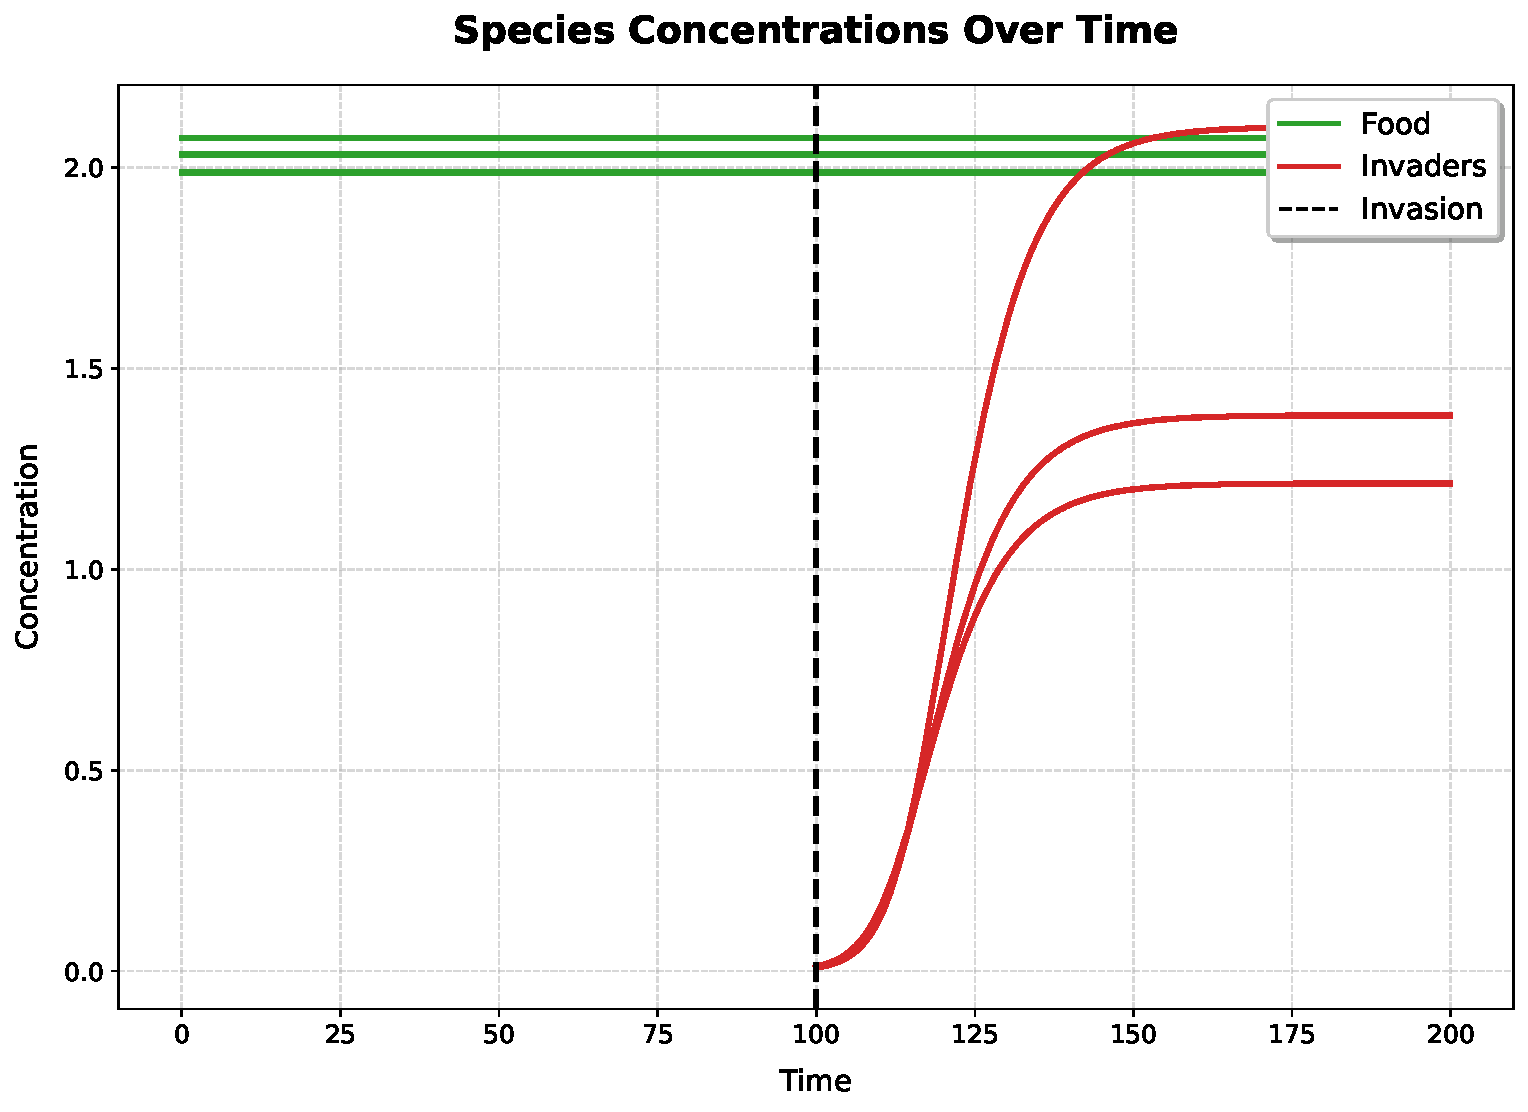
\includegraphics[width=0.6\linewidth]{Successive_species_concentrations.pdf} 
    \caption{\small{Sketch of a single "invasion", the food $N_X=3, \ N_{RX}=2$ was there until $ttot=100.0$. After that, the first $N_Y=3, \ N_{RY}=3$ arrive and autocatalytically grow}}
    \label{Fig. 9}
\end{figure}

As just seen, there is no reason to call the first $N_X$ species original ones, since their point is to keep the system out of equilibrium. In fact, the first set of invaders, can either die (or not grow enough) or grow exponentially thanks to autocatalysis. If the latter happens, after a time $ttot$, the surviving invaders will become original species, being now allowed to evolve freely but also \textbf{to be exploited and interact} with new set of invaders, that will come afterwards. Indeed, each time $ttot$ it can happen

\begin{itemize}
    \item \textbf{The set of invaders doesn't survive}
    \begin{itemize}
        \item[-] $N_X$ food species stay constant
        \item[-] The original community remains the same after the interaction with the invaders
        \item[-] A new set of $N_Y$ invaders is introduced
    \end{itemize}
    \item \textbf{The set of invaders survives}
     \begin{itemize}
        \item[-] $N_X$ food species stay constant
        \item[-] The original community is updated, the invaders become part of the original community
        \item[-] A new set of $N_Y$ invaders is introduced
    \end{itemize}
\end{itemize}
\end{comment}

In the following, we will show an example of two successful invasions into a random network. We choose $N_F=1$. After the first $ttot=150.0$ a random matrix is generated for $N_Y=3, \ N_{RY}=3$

\begin{center}
\begin{equation}
    S^{trial}_Y = \begin{pmatrix}
        0 & 1 & 0 \\
0 & 0 & 0 \\
0 & 0 & 0 \\
-1 & -1 & -1 \\
1 & 0 & 2 \\
0 & 1 & 0 \\
         \end{pmatrix}
\end{equation}
\end{center}

Meaning that the new species are reacting with the food ($F_1, \ F_2, \ F_3$) through

\begin{equation}
		\begin{split}
\ce{\textsf{Y}_1 & <--> \textsf{Y}_2 }\\ 
\ce{\textsf{Y}_1 & <--> \textsf{Y}_3 + \textsf{F}_1 }\\ 
\ce{\textsf{Y}_1 & <--> 2 \textsf{Y}_2}\\ 
\end{split} 
\end{equation}
\\

As one can see, the overall matrix will be $S=S^{trial}_Y$. This shows indeed
a Type 1 core, and when simulated, the invaders $Y$ grow. This means that they will now become part of the community, as species $X$'s

\begin{equation}
		\begin{split}
\ce{\textsf{X}_1 & <--> \textsf{X}_2 }\\ 
\ce{\textsf{X}_1 & <--> \textsf{X}_3 + \textsf{F}_1 }\\ 
\ce{\textsf{X}_1 & <--> 2 \textsf{X}_2}\\ 
\end{split} 
\end{equation}
\\

At time $t=300.0$ the second (or the first real) invasion starts. The proposed random matrix is 

\begin{center}
\begin{equation}
    S^{trial}_Y = \begin{pmatrix}
0 & 0 & 0 \\
0 & 0 & 1 \\
0 & 0 & 0 \\
0 & 0 & -1 \\
0 & 0 & 0 \\
0 & 0 & 0 \\
0 & 0 & 0 \\
1 & 2 & -1 \\
-1 & -1 & 1 \\
\end{pmatrix}
\end{equation}
\end{center}

Meaning the new proposed reactions now are

\begin{equation}
		\begin{split}
\ce{\textsf{Y}_3 & <--> \textsf{Y}_2 }\\ 
\ce{\textsf{Y}_2 & <--> 2\textsf{Y}_3}\\ 
\ce{\textsf{X}_1 + \textsf{Y}_2 & <--> \textsf{Y}_3 + \textsf{F}_2}\\ 
\end{split} 
\end{equation}
\\

Thanks to autocatalysis, this new set of invaders manages to grow: the new $Y$ species will become part of the original community

\begin{center}
\begin{equation}
    S = \begin{pmatrix}
        \begin{pmatrix}
            S_X \\ \\
            \pmb{0}
        \end{pmatrix}, & S_Y
    \end{pmatrix} = \begin{pmatrix}
0 & 1 & 0 & 0 & 0 & 0 \\
0 & 0 & 0 & 0 & 0 & 1 \\
0 & 0 & 0 & 0 & 0 & 0 \\
-1 & -1 & -1 & 0 & 0 & -1 \\
1 & 0 & 2 & 0 & 0 & 0 \\
0 & 1 & 0 & 0 & 0 & 0 \\
0 & 0 & 0 & 0 & 0 & 0 \\
0 & 0 & 0 & 1 & 2 & -1 \\
0 & 0 & 0 & -1 & -1 & 1 \\
\end{pmatrix}
\end{equation}
\end{center}

Thus, the community becomes

\begin{equation}
		\begin{split}
\ce{\textsf{X}_1 & <--> \textsf{X}_2 }\\ 
\ce{\textsf{X}_1 & <--> \textsf{X}_3 + \textsf{F}_1 }\\ 
\ce{\textsf{X}_1 & <--> 2 \textsf{X}_2}\\ 
\ce{\textsf{X}_6 & <--> \textsf{X}_5 }\\ 
\ce{\textsf{X}_5 & <--> 2\textsf{X}_6}\\ 
\ce{\textsf{X}_1 + \textsf{X}_5 & <--> \textsf{X}_6 + \textsf{F}_2}\\ 
\end{split} 
\end{equation}
\\

The result of the simulation of such a network are shown in Fig. \ref{Fig. 10}

\begin{figure}[H]
    \centering
    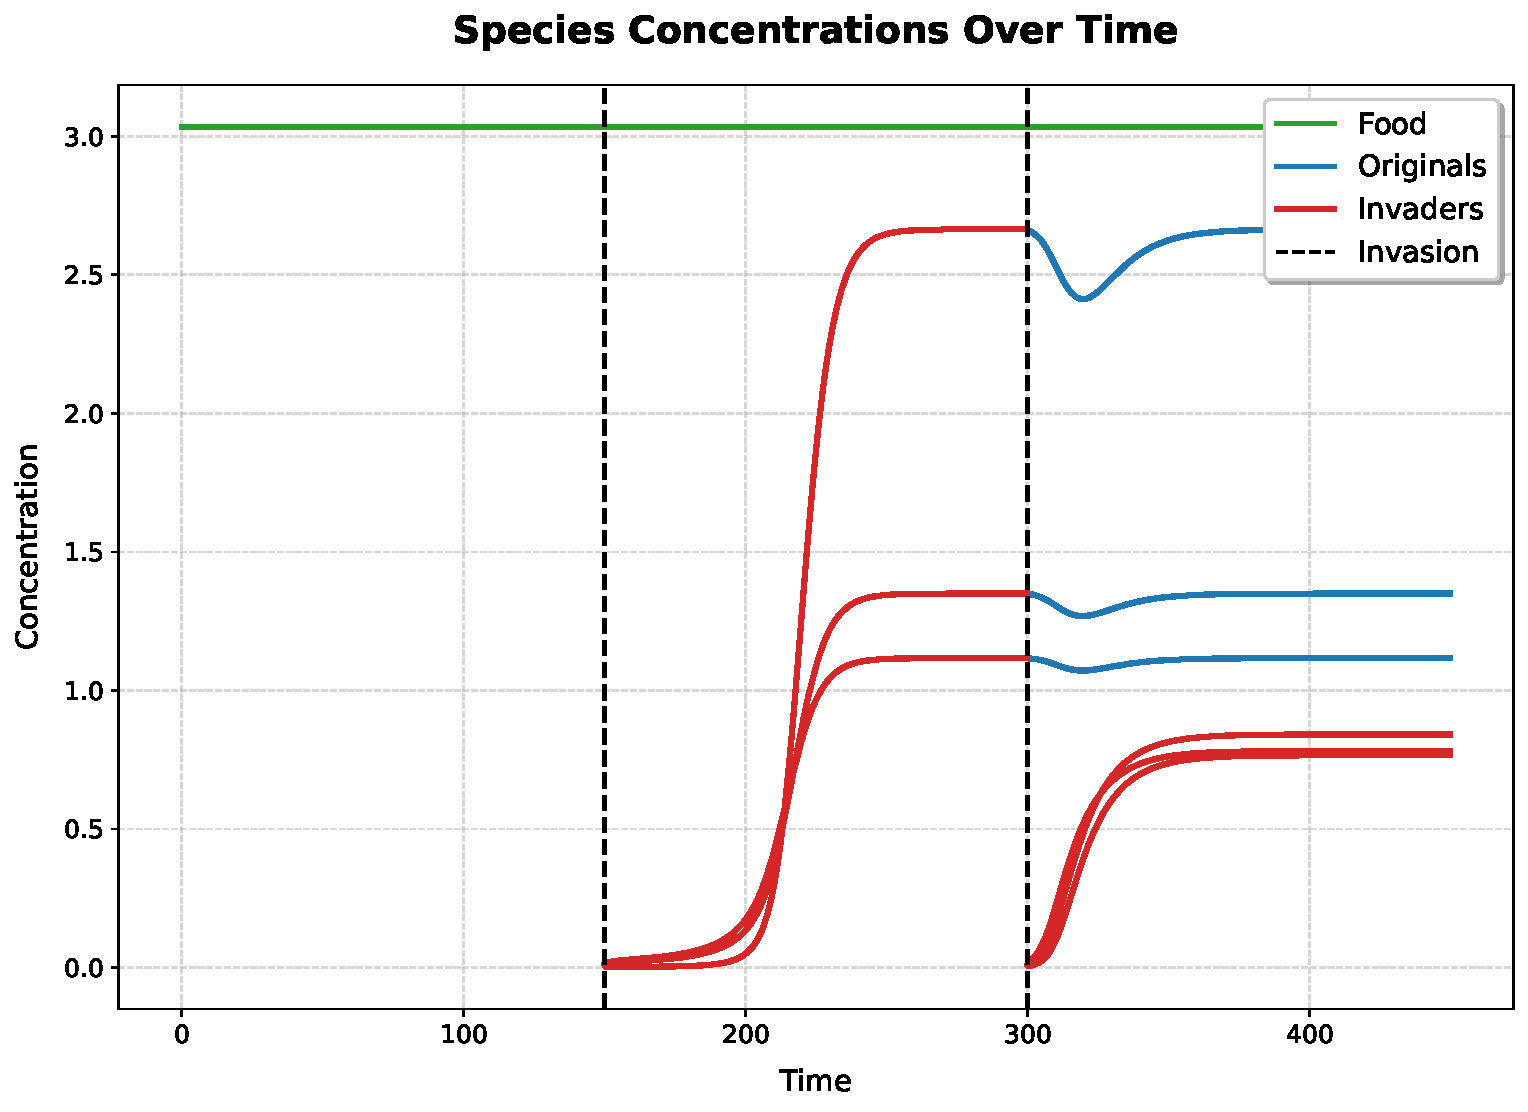
\includegraphics[width=0.6\linewidth]{Successive_species_concentrations_TRIAL.pdf} 
    \caption{\small{Sketch of two invasions, the food $F_1$ was alone in the environment until $ttot=150.0$. After that, the first $N_Y=3, \ N_{RY}=3$ arrive and autocatalytically grow, surviving. Another set of invaders is introduced at $t=300.0$. Now they evolve and grow exploiting the previous set of invaders, which became original species.}}
    \label{Fig. 10}
\end{figure}

We will analyze the behavior of the total population over time, the number of cores produced each invasion, the stoichiometry and their correlation with successful surviving rates. Furthermore, we'll look at the currents for each reaction at steady state, after each invasion, as well as thermodynamic quantities when the community settles to a stable steady state.

\subsection{Groups of parasitic invaders: an example}

We will consider an example of a network that starts with $N_F=3$ and gets invaded every $ttot = 100.0$ by a number of invaders $N_Y = 3$ who come along with $N_RY = 3$ reactions led by MAL. Forward rate constants are sampled from a uniform distribution centered in $2$, and $\mu_0$'s are taken from a uniform one between $-1$ and $1$. The system undergoes a number of such invasions sets by $Invasions = 100$. The group of invaders is set to be a $parasite$, so that the set of possible proposed reactions will span among:
\begin{equation}
		\begin{split}
\ce{\textsf{Y}_i & <--> \textsf{Y}_j } \quad \quad i \neq j \\ 
\ce{\textsf{X}_i + \textsf{Y}_j & <--> \textsf{Y}_k + \textsf{Y}_l } \quad \quad j \neq k,l \\ 
\ce{\textsf{X}_l + \textsf{Y}_i & <--> \textsf{Y}_j + \textsf{X}_m } \quad \quad i \neq j , \ l \neq m\\ 
\end{split} 
\end{equation}

where $X_i$ is an original species from the community if $i>N_F$, or it's chemostated food when $i \le N_F$. The concentration of the food species at $t=0$ will be sampled from a uniform distribution centered in $3.0$ whereas the cooncentration of the invaders when they are introduced in the system will be sampled around a value of $0.01$. The invasion is considered successful if the sum of the newcomers reaches a threshold of $0.2$ during the time $ttot$, when we also expect the system to relax before a new invasion.

The results of the dynamics are shown in the following:

\begin{figure}[H]
    \centering
    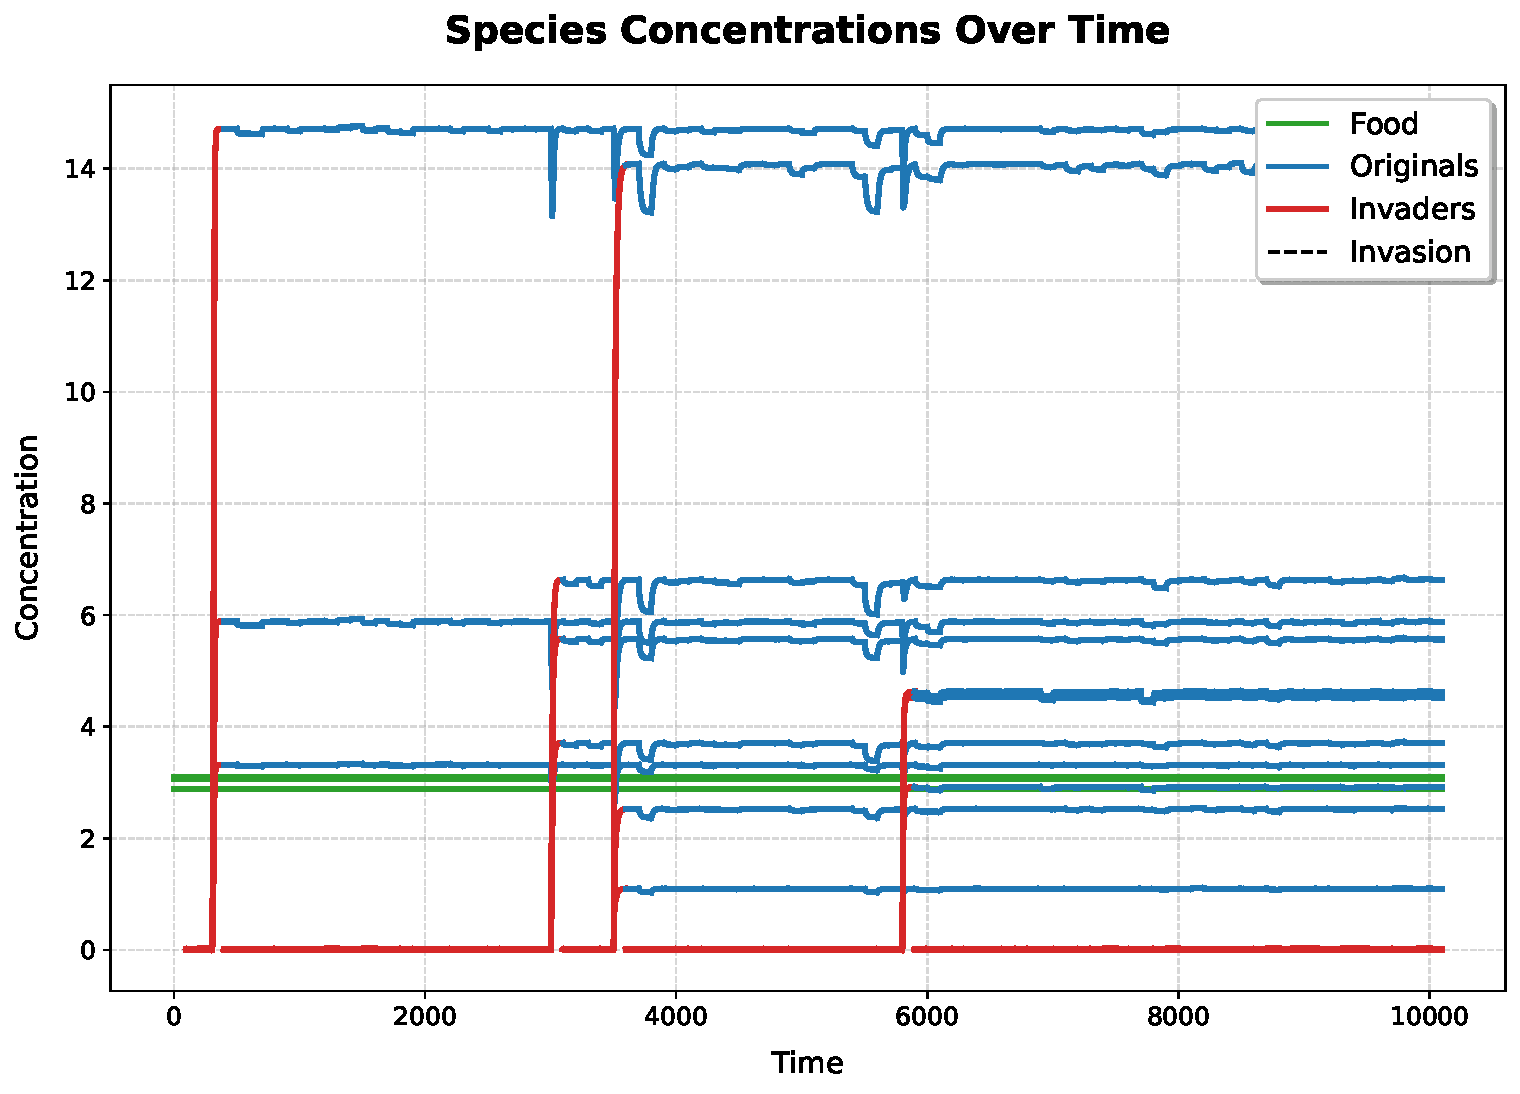
\includegraphics[width=0.6\linewidth]{Successive_species_concentrations_2.pdf} 
    \caption{\small{Evolution of invaders (red curves) introduced each $ttot=100$ and of original species (blue curves). If the group of invaders survive then it becomes part of the original community. Food species are constant and shown in green.}}
    \label{Fig. 11}
\end{figure}

The stoichiometric matrix of such a system of parasitic invaders, after $100$ trial invasions with only $4$ successful ones will be:

\newenvironment{mpmatrix}{\begin{medsize}\begin{pmatrix}}%
    {\end{pmatrix}\end{medsize}}%

\[S=
\begin{mpmatrix}
0 & 0 & 0 & 0 & 0 & 0 & -1 & 0 & 0 & 0 & 0 & 0 & 0 & 0 & 0 \\
0 & 0 & 0 & 0 & 0 & 0 & 0 & 0 & 0 & 0 & 0 & 0 & 0 & 0 & 0 \\
0 & 0 & -1 & 0 & 0 & 0 & 0 & 0 & 0 & 0 & 0 & 0 & 0 & 0 & 0 \\
-1 & 0 & 1 & 0 & 0 & 0 & 0 & 0 & 0 & -1 & 0 & 0 & 0 & -1 & 0 \\
1 & 1 & 1 & -1 & 0 & 0 & 0 & 0 & 0 & 0 & 0 & 0 & 0 & 0 & 0 \\
0 & -1 & -1 & 0 & 0 & 0 & 0 & 0 & 0 & 0 & 0 & 0 & 0 & 0 & 0 \\
0 & 0 & 0 & 0 & 0 & -1 & 0 & 0 & 0 & 0 & 0 & 0 & 0 & 0 & 0 \\
0 & 0 & 0 & 2 & -1 & 0 & 0 & -1 & 0 & 0 & 0 & 0 & 0 & 0 & 0 \\
0 & 0 & 0 & -1 & 1 & 1 & 0 & 0 & 0 & 0 & 0 & 0 & 0 & 0 & 0 \\
0 & 0 & 0 & 0 & 0 & 0 & 1 & 1 & 0 & 0 & 0 & 0 & 0 & 0 & 0 \\
0 & 0 & 0 & 0 & 0 & 0 & 0 & 1 & 1 & 0 & 0 & 0 & 0 & 0 & 0 \\
0 & 0 & 0 & 0 & 0 & 0 & -1 & -1 & -1 & 0 & 0 & 0 & 0 & 0 & 0 \\
0 & 0 & 0 & 0 & 0 & 0 & 0 & 0 & 0 & 2 & 1 & -1 & 0 & 0 & 0 \\
0 & 0 & 0 & 0 & 0 & 0 & 0 & 0 & 0 & 0 & -1 & 0 & 0 & 0 & 0 \\
0 & 0 & 0 & 0 & 0 & 0 & 0 & 0 & 0 & -1 & 0 & 1 & 0 & 0 & 0 \\
0 & 0 & 0 & 0 & 0 & 0 & 0 & 0 & 0 & 0 & 0 & 0 & 1 & 1 & 1 \\
0 & 0 & 0 & 0 & 0 & 0 & 0 & 0 & 0 & 0 & 0 & 0 & -1 & -1 & -1 \\
0 & 0 & 0 & 0 & 0 & 0 & 0 & 0 & 0 & 0 & 0 & 0 & 0 & 0 & 0
\end{mpmatrix}
\]




At the end of the process, all $Y$' s became $X$' s, so we shall refer to them this way when showing the reactions.

\begin{equation}
		\begin{split}
\ce{\textsf{X}_1 & <--> \textsf{X}_2 }\\ 
\ce{\textsf{X}_3 & <--> \textsf{X}_2}\\ 
\ce{\textsf{F}_3 + \textsf{X}_3 & <--> \textsf{X}_1 + \textsf{X}_2}\\ 
\ce{\textsf{X}_2 + \textsf{X}_6 & <--> 2 \textsf{X}_5 }\\ 
\ce{\textsf{X}_5 & <--> \textsf{X}_6}\\ 
\ce{\textsf{X}_4 & <--> \textsf{X}_6}\\ 
\ce{\textsf{F}_1 + \textsf{X}_9 & <--> \textsf{X}_7}\\ 
\ce{\textsf{X}_5 + \textsf{X}_9 & <--> \textsf{X}_7 + \textsf{X}_8}\\ 
\ce{\textsf{X}_9 & <--> \textsf{X}_8}\\ 
\ce{\textsf{X}_{12} + \textsf{X}_1 & <--> 2 \textsf{X}_10}\\ 
\ce{\textsf{X}_{11} & <--> \textsf{X}_{10}}\\ 
\ce{\textsf{X}_{10} & <--> \textsf{X}_{12}}\\ 
\ce{\textsf{X}_{14} & <--> \textsf{X}_{13}}\\ 
\ce{\textsf{X}_{1} + \textsf{X}_{11} & <--> \textsf{X}_{10}}\\ 
\ce{\textsf{X}_{14} & <--> \textsf{X}_{13}}\\  
\end{split} 
\end{equation}
\\

At steady state, when the $100$ invasions stop, the systems shows a distribution of currents and affinities peaked around $0$, with just a few reactions being out of equilibrium:

\begin{figure}[H]
    \centering
    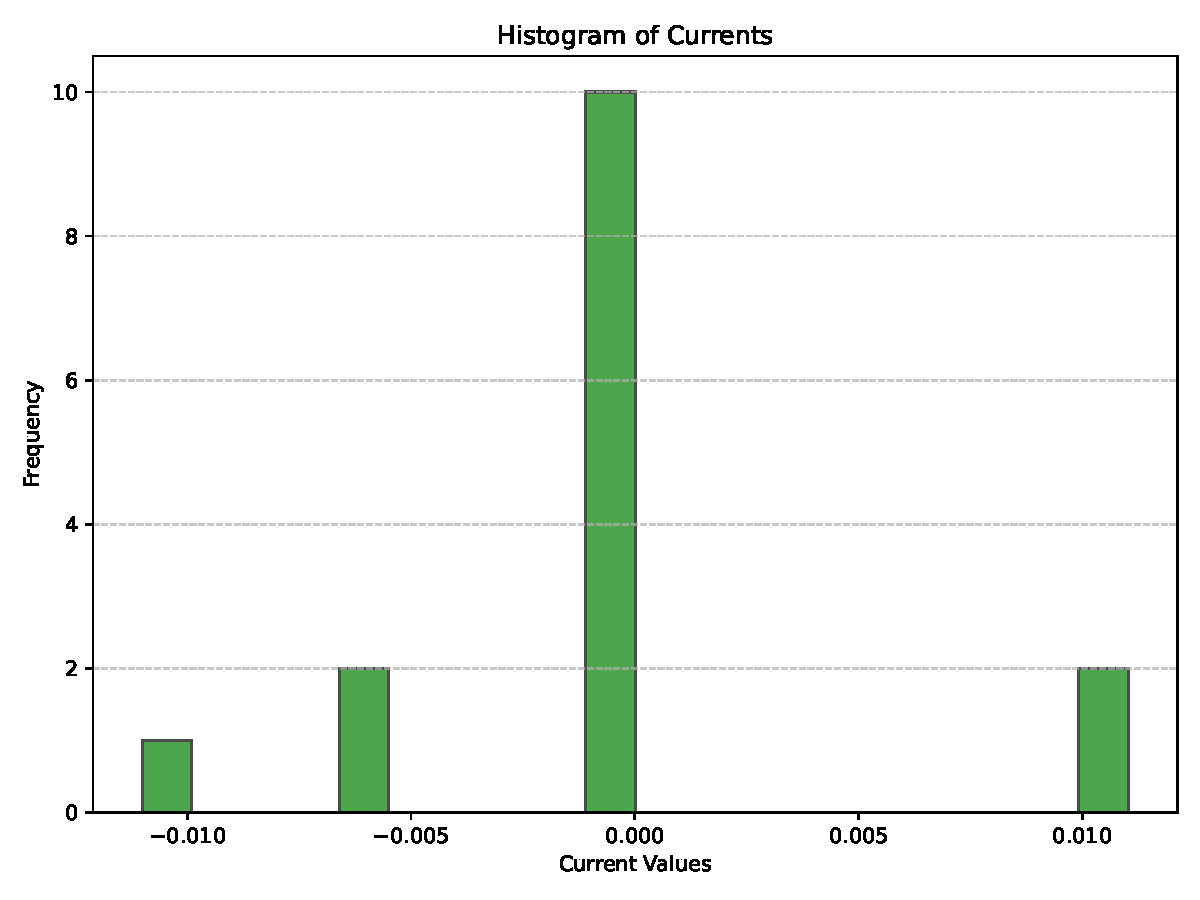
\includegraphics[width=0.45\linewidth]{Currents.pdf}
    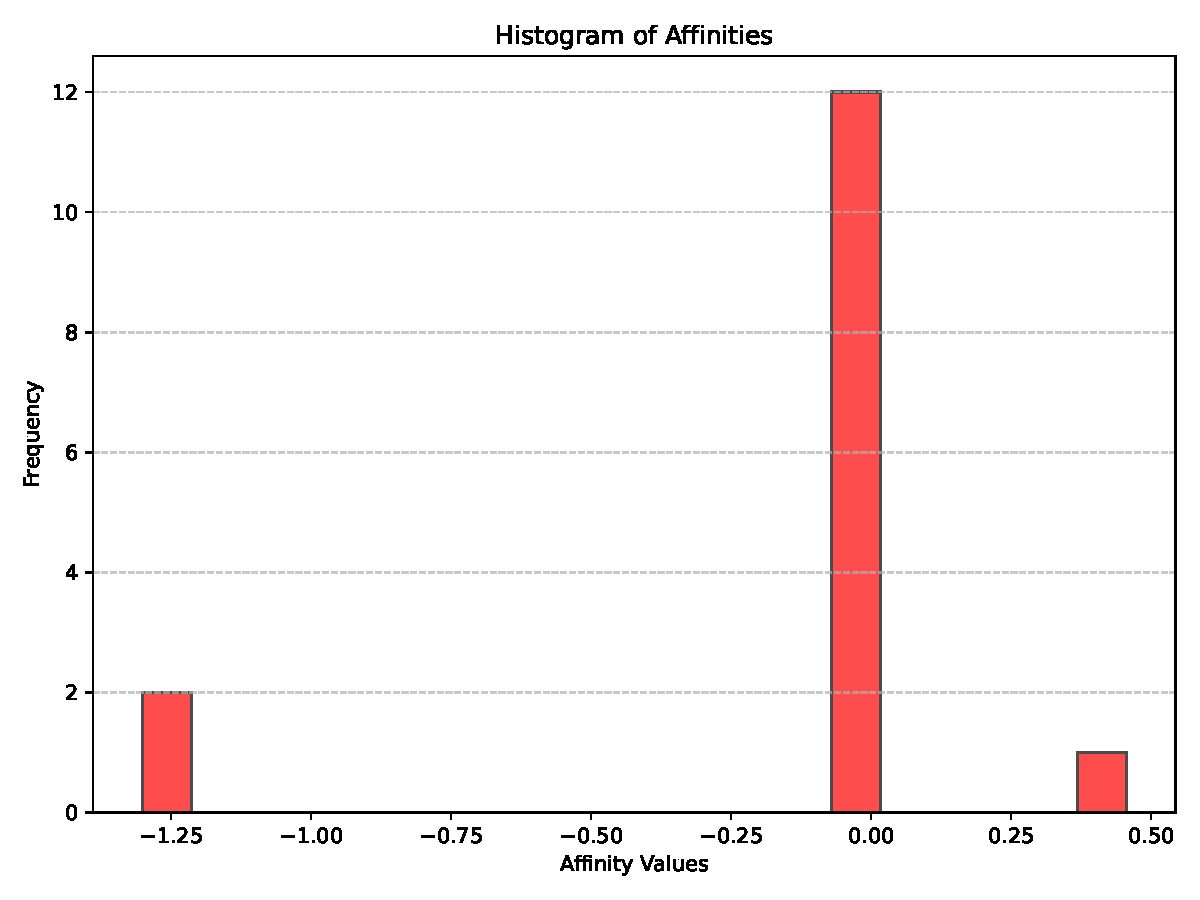
\includegraphics[width=0.45\linewidth]{Affinities.pdf} 
    \caption{\small{Currents (left plot) and affinities (right plot) after $100$ invasions and $15$ reversible reactions. Only few of them are out of equilibrium. }}
    \label{Fig. 12}
\end{figure}

From an evolutionary point of view, we can analyze the behavior of the growing total population, which will present typical plateaus as shown in \cite{4} 

\begin{figure}[H]
    \centering
    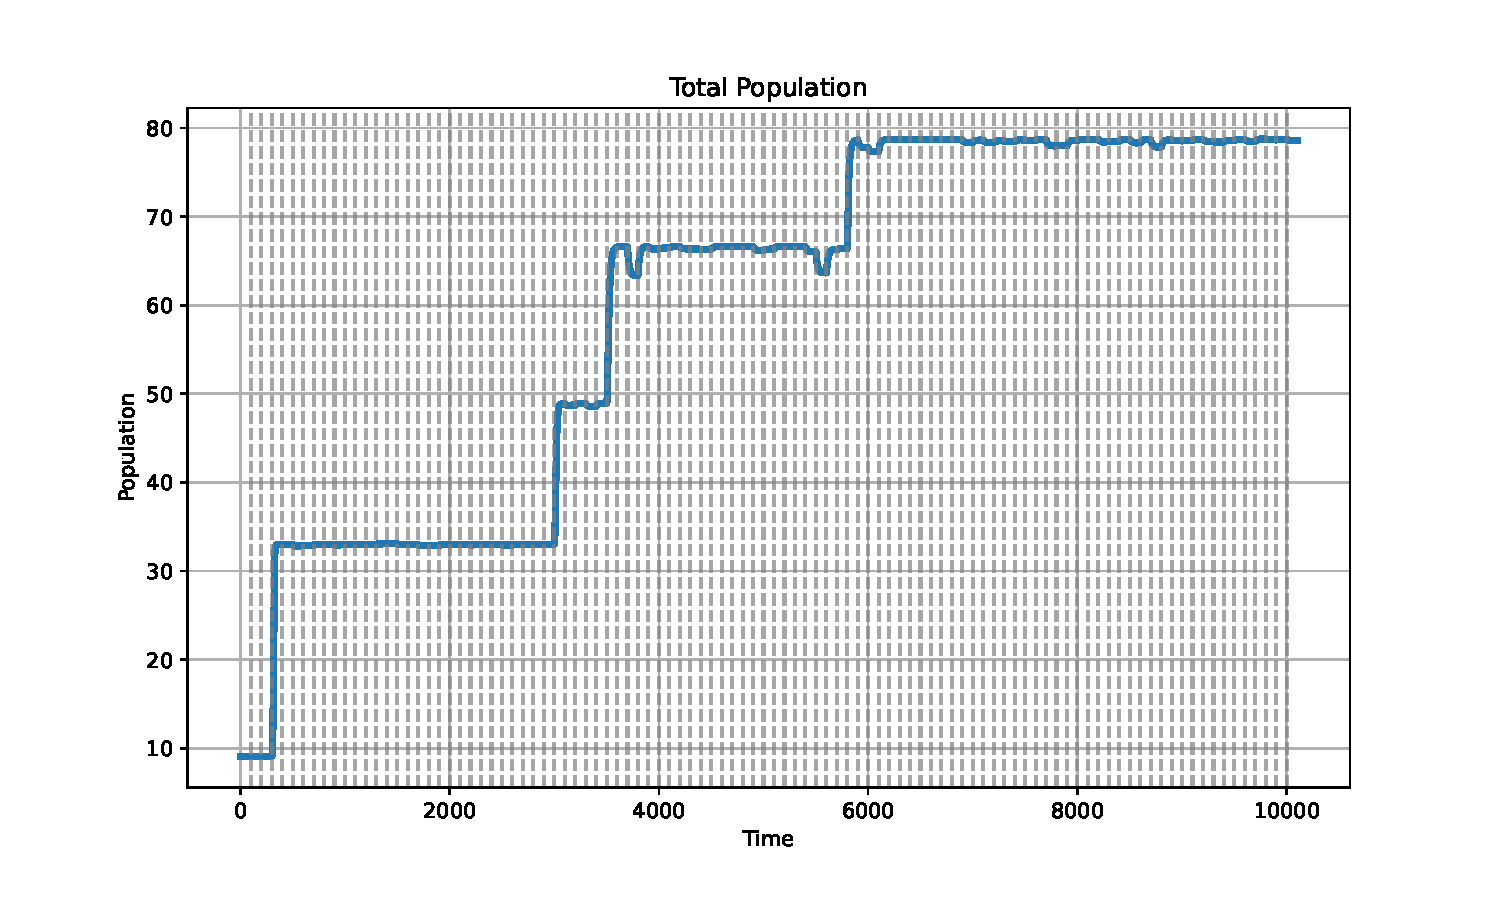
\includegraphics[width=0.6\linewidth]{Invasions_total.pdf}
    \caption{\small{Total population of original species and invaders, growing with time. The four successful invasions can be easily identified.}}
    \label{Fig. 13}
\end{figure}

To conclude, we analyze the emergency of cores in the system and their relationship with the increase of species over time:

\begin{figure}[H]
    \centering
    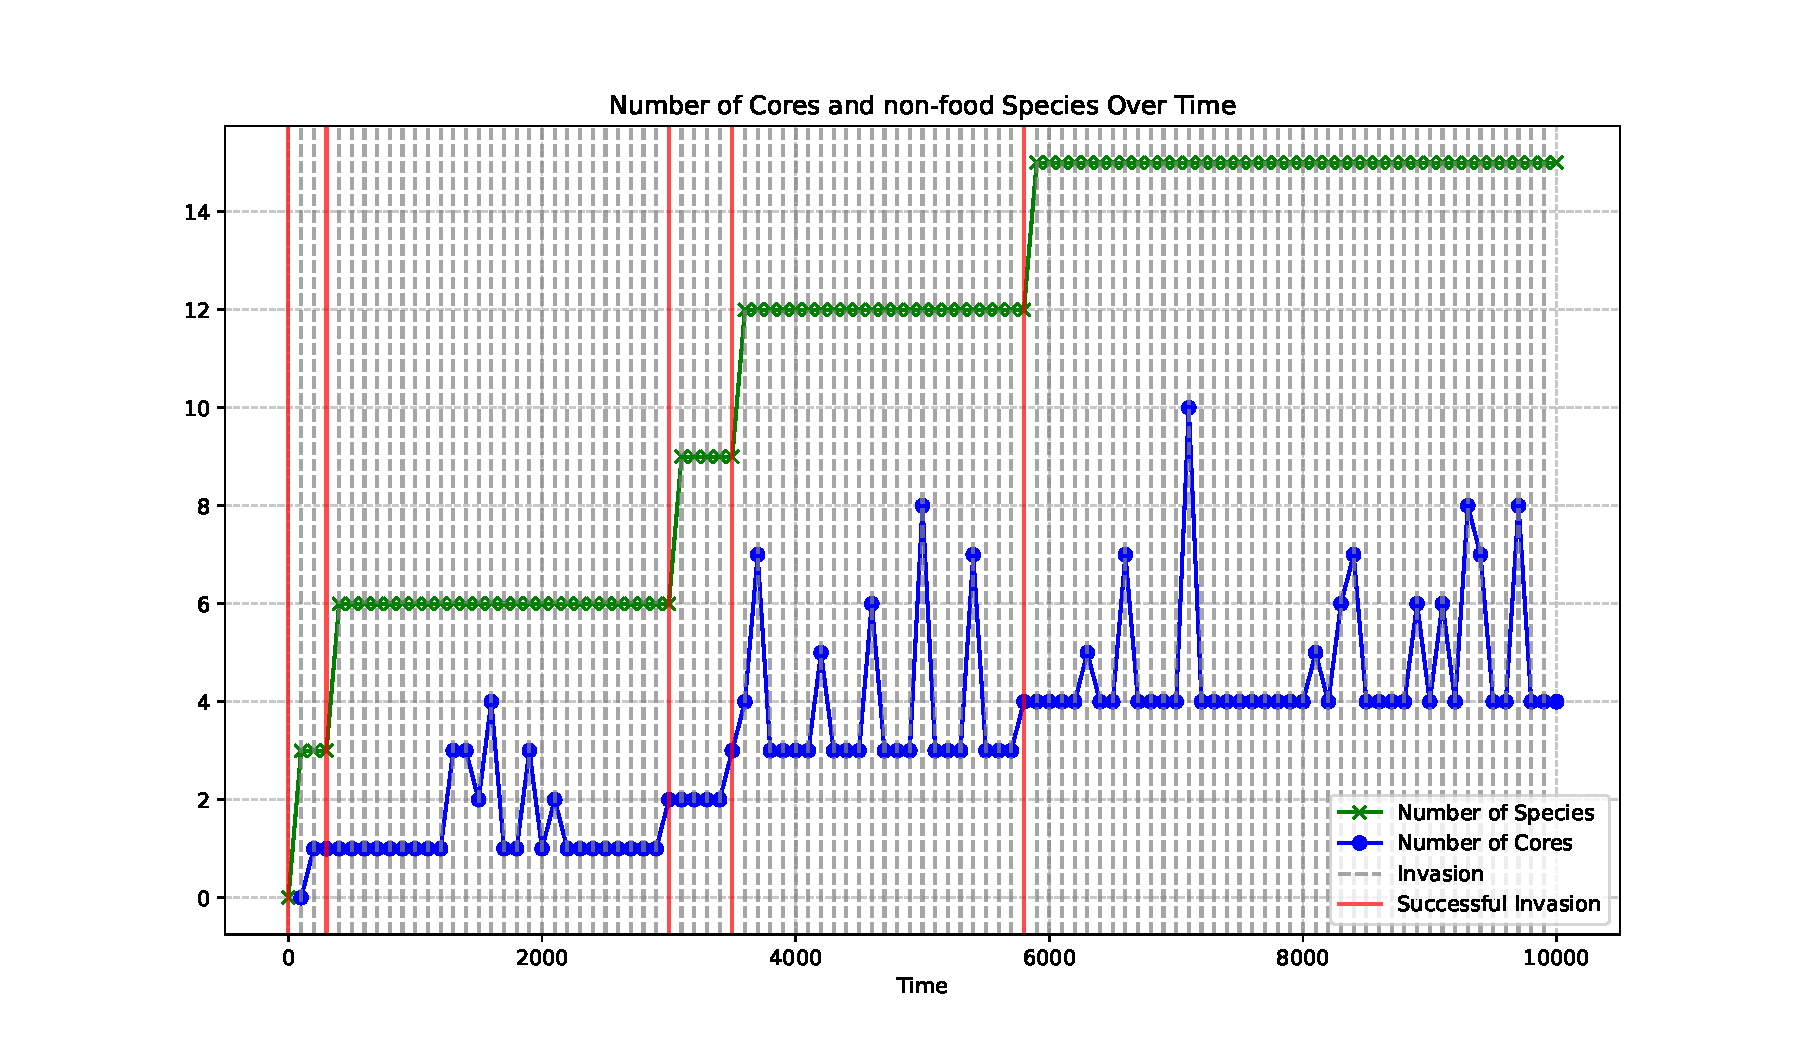
\includegraphics[width=0.6\linewidth]{Cores_species.pdf}
    \caption{\small{Green line shows the number of (non-food) species increasing over time due to successful invasions. Blue line is instead showing the number of cores associated with the network at that time. }}
    \label{Fig. 14}
\end{figure}

From Fig. \ref{Fig. 14} it's clear that for an higher number of species, there is, on average, an higher number of potential cores, but it's also easy to see that not always more cores correspond to higher probabilities of successful invasion. Indeed, all the $4$ (not considering the first) successful ones are associated with the increase of just one single core in the network, provided it to be a good kinetic candidate. Whenever we have peaks in the number of cores instead, probably due to competition between them, the invasion is more likely not to succeede. 


\subsection{Groups of competitive invaders: an example}

As before, we'll consider an example of a network that starts with $N_F=3$ and gets invaded every $ttot = 100.0$ by a number of invaders $N_Y = 3$ who come along with $N_{RY} = 3$ reactions led by MAL. We will now simulate a smaller number of invasions $Invasions = 20$, since the autocatalytic feature of the invaders in this case will produce a lot of cores and huge networks. In fact, the group of invaders is set to be $competing$ against the $X$ species, so that the set of possible proposed reactions will span among:
\begin{equation}
		\begin{split}
\ce{\textsf{Y}_i & <--> \textsf{Y}_j } \quad \quad i \neq j \\ 
\ce{\textsf{Y}_i & <--> \textsf{Y}_j + \textsf{Y}_k } \quad \quad i \neq j,k \\
\ce{\textsf{F}_i + \textsf{Y}_j & <--> \textsf{Y}_k + \textsf{Y}_l } \quad \quad j \neq k,l \\ 
\ce{\textsf{F}_l + \textsf{Y}_i & <--> \textsf{Y}_j + \textsf{F}_m } \quad \quad i \neq j , \ l \neq m\\ 
\end{split} 
\end{equation}
where $X_i$ is an original species from the community if $i>N_F$, or it's chemostated food when $i \le N_F$. As before, $\left[\mathbf{F}\right](t=0) \sim 3*U(0.95,1.05)$ and  $\left[\mathbf{Y}\right](t=0) \sim 0.01*U(0.95,1.05)$. The invasion is considered successful if the sum of the newcomers reaches a threshold of $0.2$ during the time $ttot$, when we also expect the system to relax before a new invasion. \\

We expect this system to produce way more cores than the \textbf{parasitic} case, since $Y$ species are now capable of reproduce themselves on their own. We emphasize this to be the reason of the choice of only $20$ invasions.


The results of the dynamics are shown in the following:

\begin{figure}[H]
    \centering
    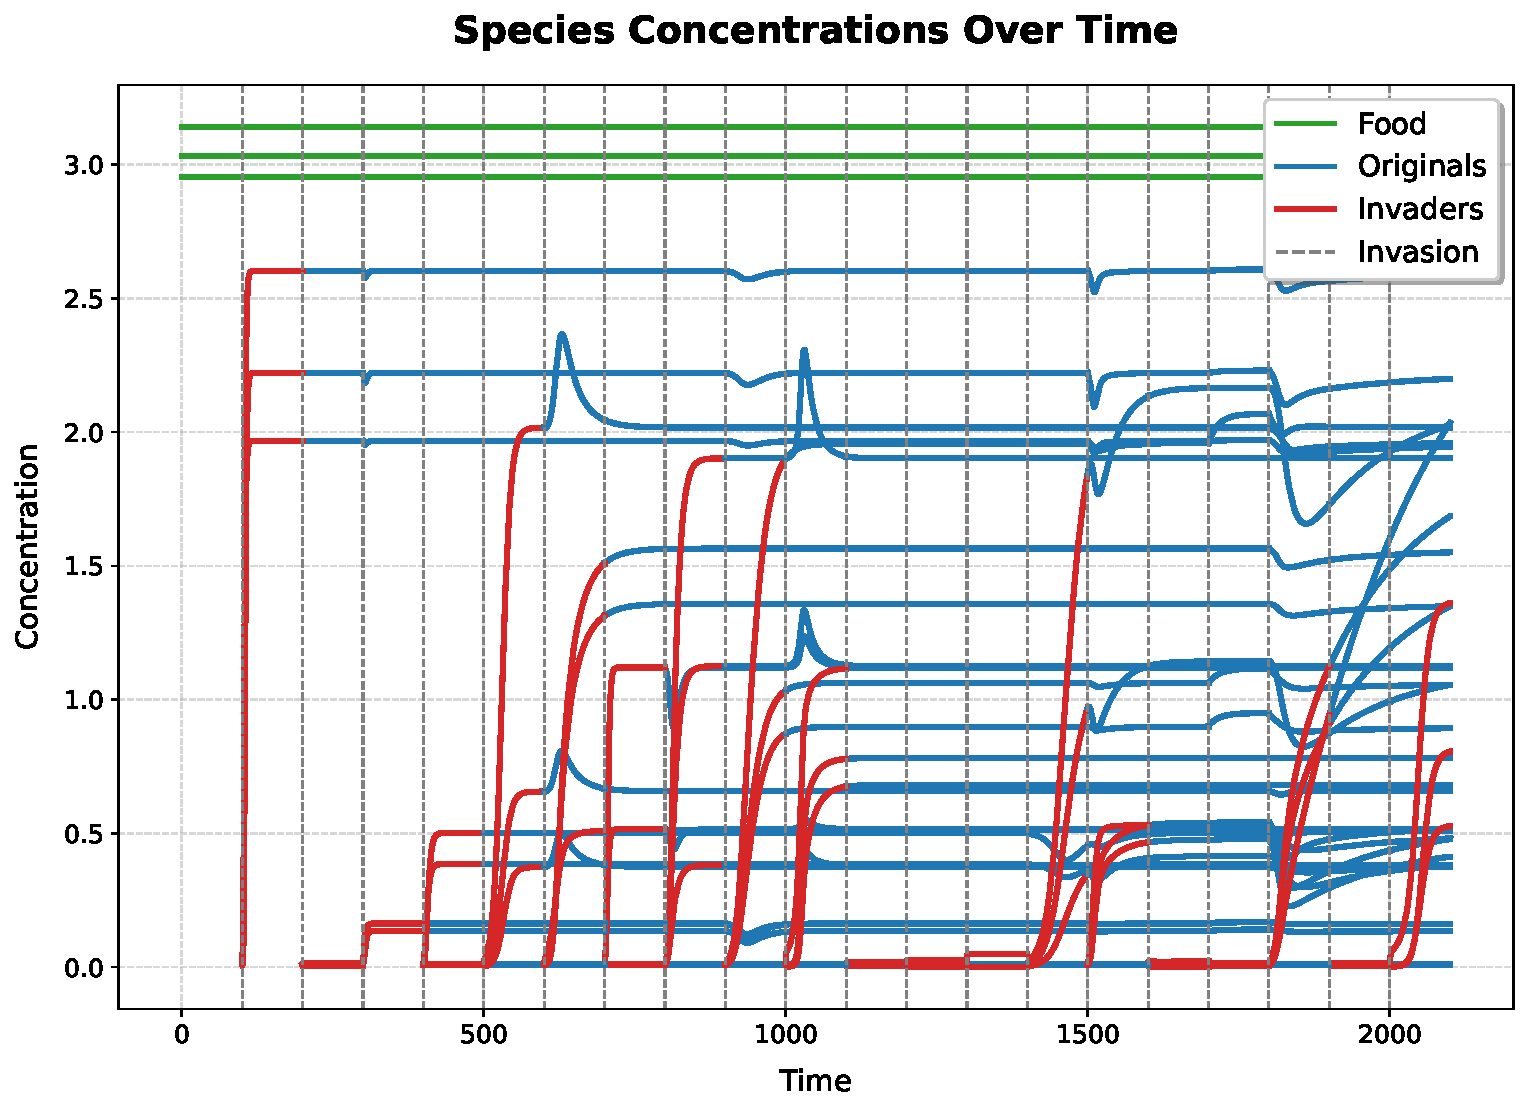
\includegraphics[width=0.6\linewidth]{Successive_species_concentrations_auto.pdf} 
    \caption{\small{Evolution of invaders (red curves) introduced each $ttot=100$ and of original species (blue curves). If the group of invaders survive then it becomes part of the original community. Food species are constant and shown in green. Competitive case}}
    \label{Fig. 15}
\end{figure}

As expected, there is way more chance of survival with respect to the \textbf{parasitic} case. In the case of Fig. \ref{Fig. 11} the survival rate has shown to be $\frac{4}{100}$, whereas in this \textbf{competitive} case we ended up with $\frac{13}{20}$. The stoichiometric matrix of such a system of competitive invaders, after $20$ trial invasions with $13$ successful ones will be a $42\times 39$ matrix, indeed describing 39 reversible reactions. For obvious reasons, we're not showing them in the following. \\ Nevertheles, we can look at the distributions of currents and affinities at steady state:

\begin{figure}[H]
	\centering
	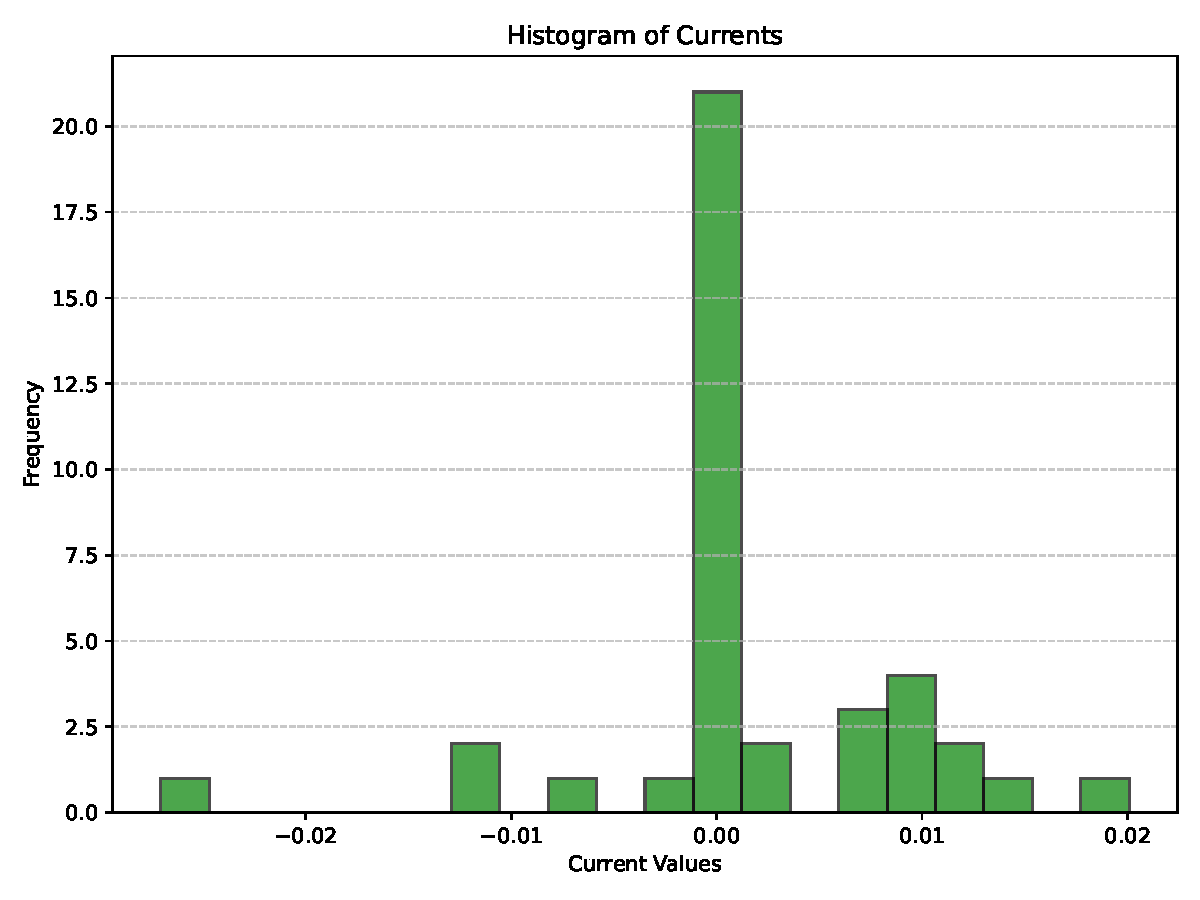
\includegraphics[width=0.45\linewidth]{Currents_auto.pdf}
	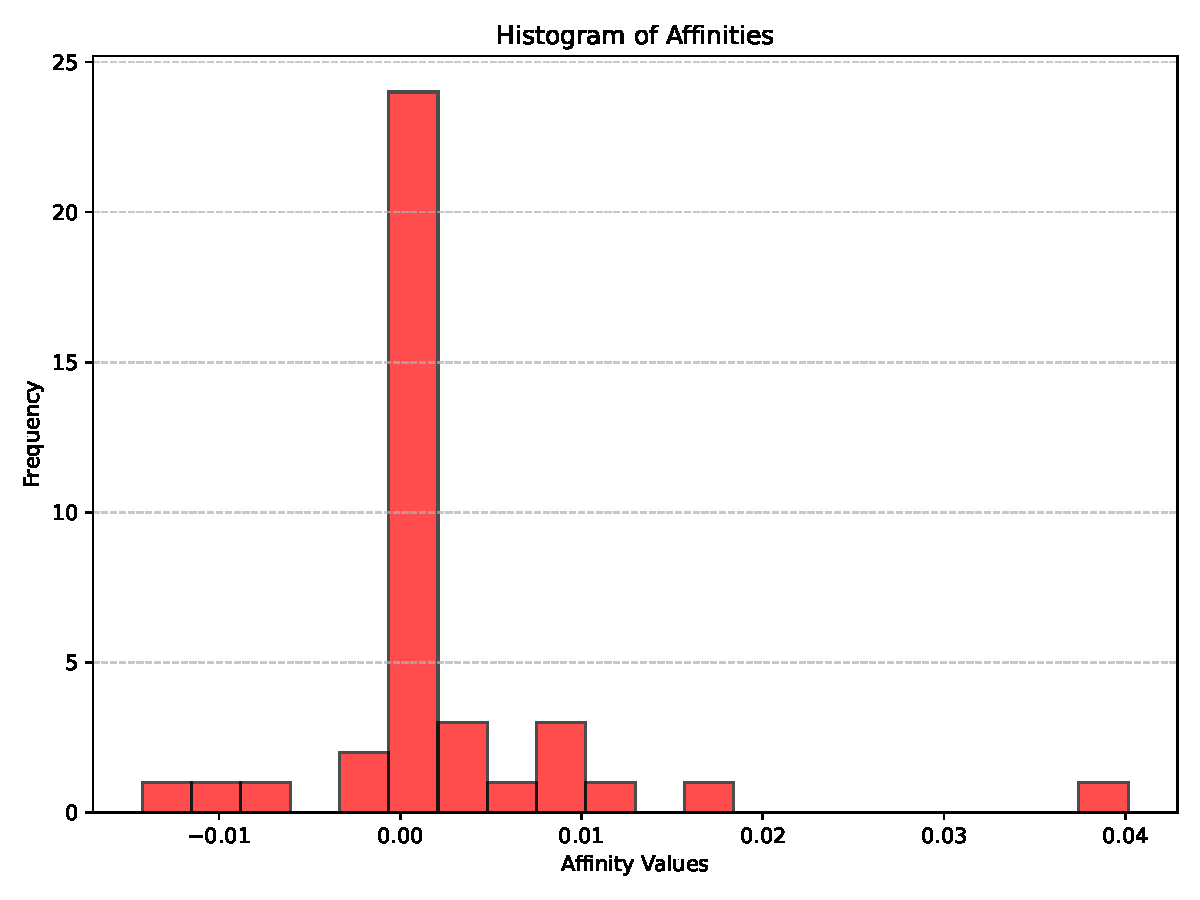
\includegraphics[width=0.45\linewidth]{Affinities_auto.pdf} 
	\caption{\small{Currents (left plot) and affinities (right plot) after $20$ invasions and $39$ reversible reactions. Only few of them are out of equilibrium. }}
	\label{Fig. 16}
\end{figure}

From an evolutionary point of view, we can analyze the behavior of the growing total population

\begin{figure}[H]
	\centering
	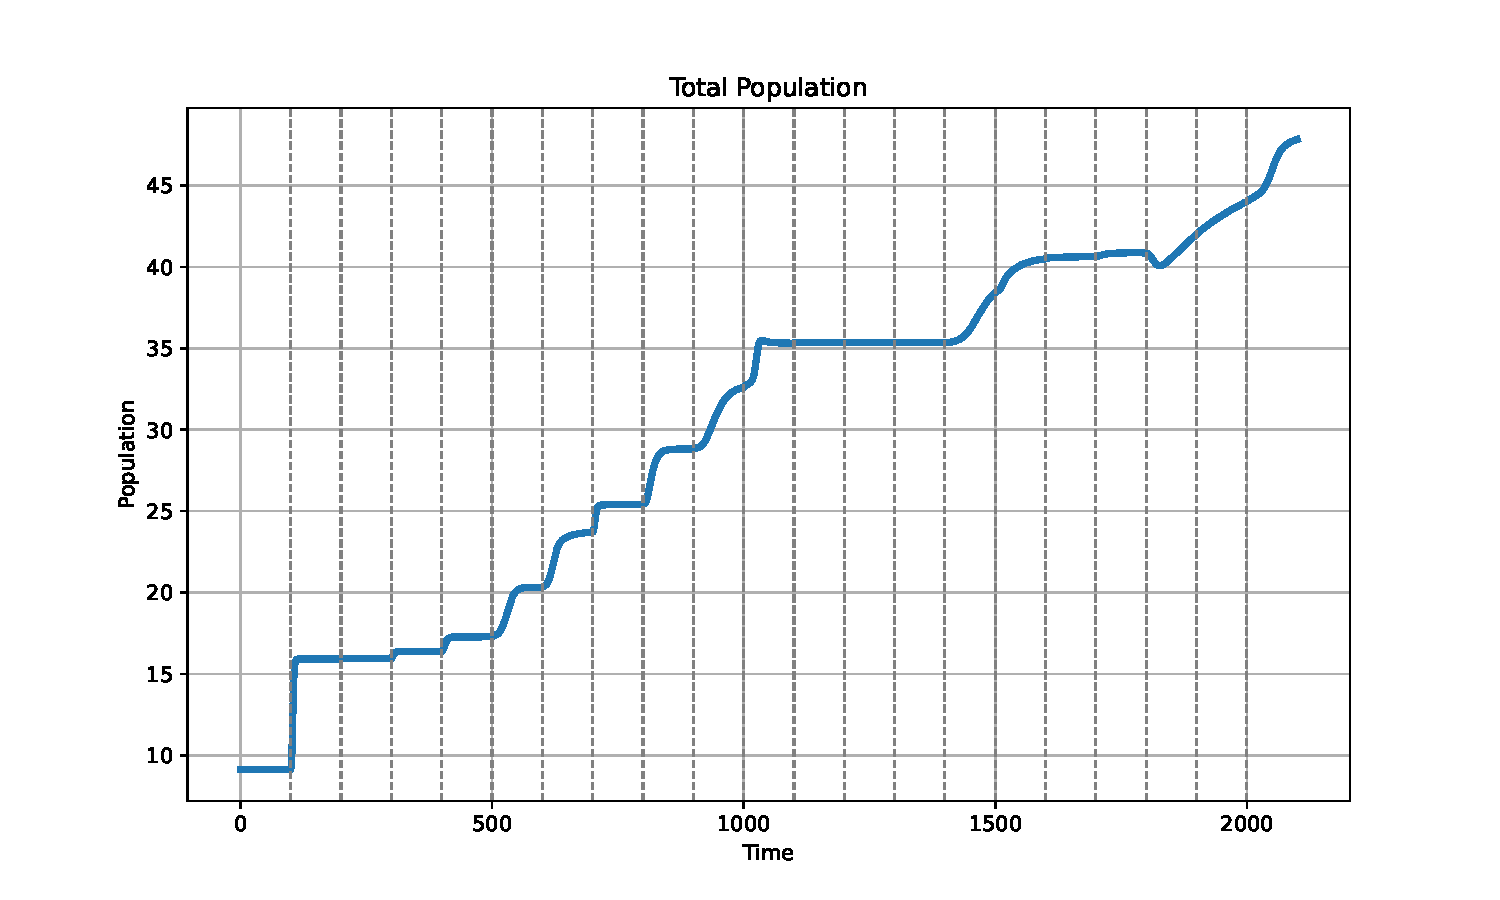
\includegraphics[width=0.6\linewidth]{Invasions_total_auto.pdf}
	\caption{\small{Total population of original species and invaders, growing with time.}}
	\label{Fig. 17}
\end{figure}

To conclude, we analyze the emergency of cores in the system and their relationship with the increase of species over time:

\begin{figure}[H]
	\centering
	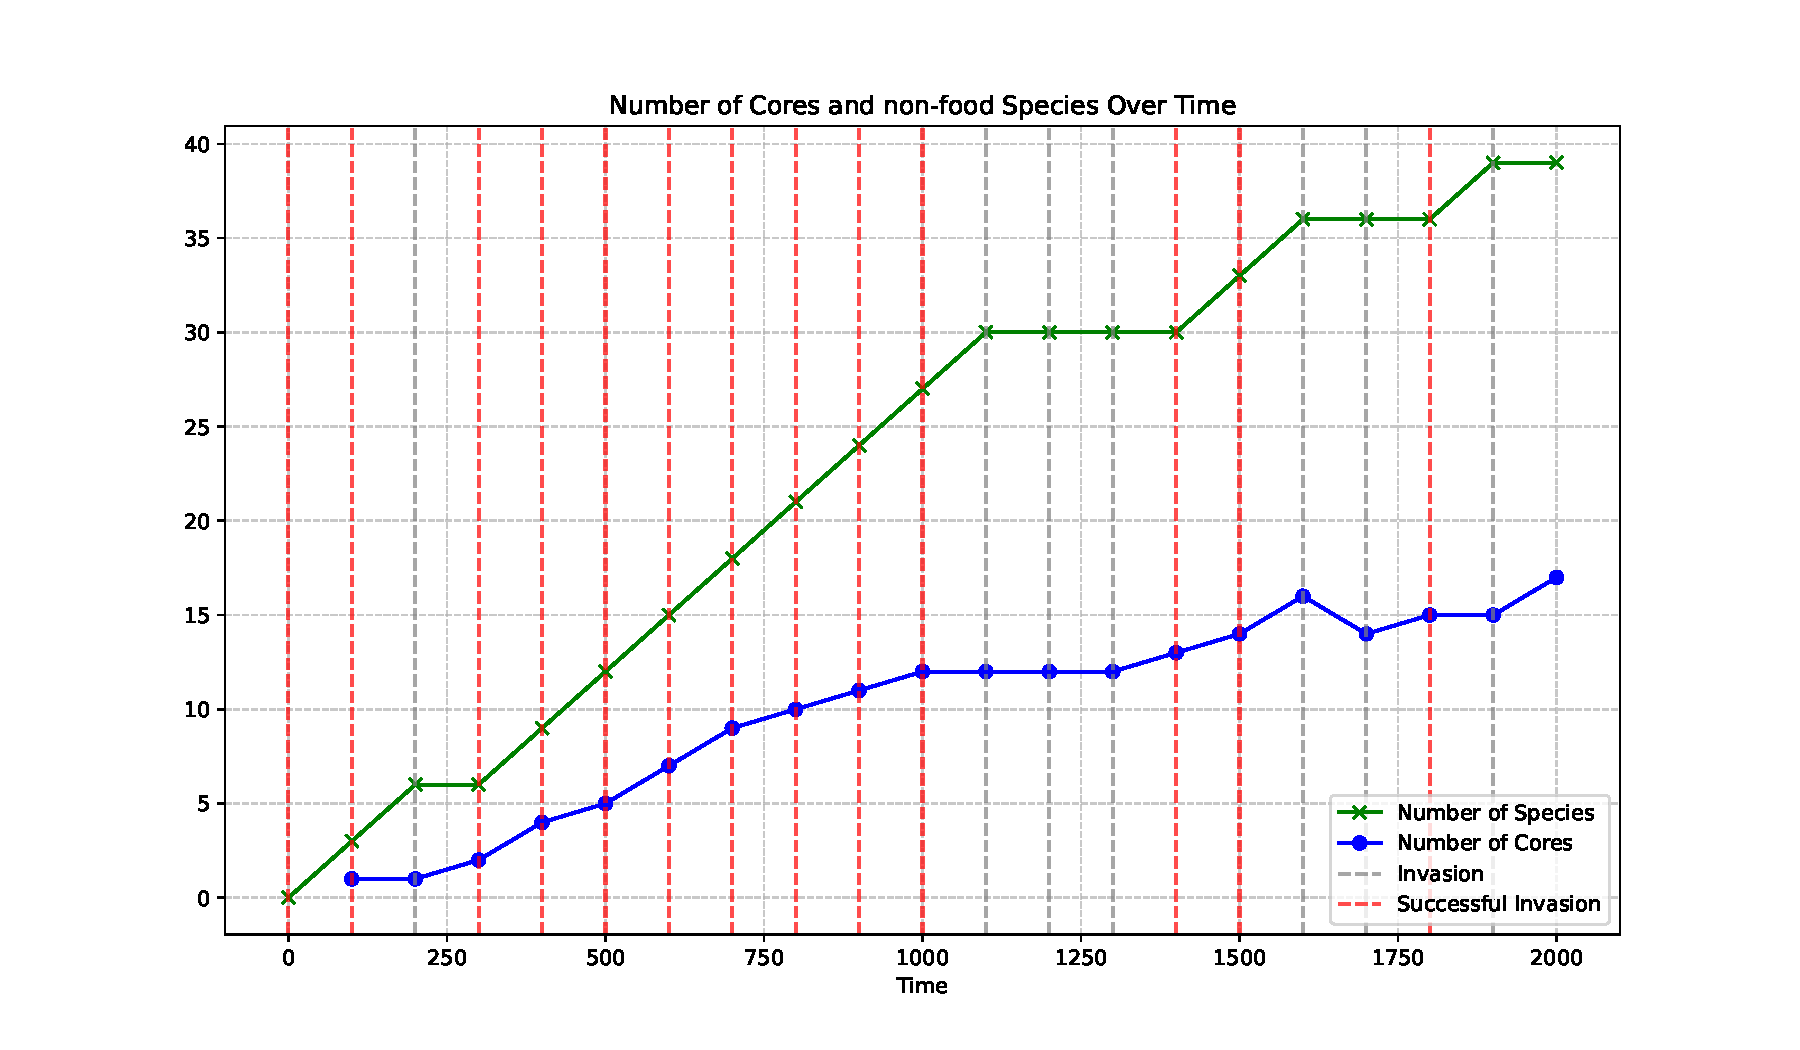
\includegraphics[width=0.6\linewidth]{Cores_species_auto.pdf}
	\caption{\small{Green line shows the number of (non-food) species increasing over time due to successful invasions. Blue line is instead showing the number of cores associated with the network at that time. }}
	\label{Fig. 18}
\end{figure}



\printbibliography


\end{document}
